\chapter{Introduction}		% chapter 1
\label{introchap}		% for reference (\ref{introchap})


Humorous fable by Horace Lamb, British physicist and applied mathematician, in 1932 just two years before his death in 1934 goes as follows: ``I am an old man now, and when I die and go to heaven there are two matters on which I hope for enlightenment. One is quantum electrodynamics, and the other is the turbulent motion of fluids. And about the former I am rather optimistic.''


In the words of the legendary Nobel Prize-winning physicist, Richard Feynman, ``Turbulence is the last great unsolved problem of classical physics.''


George Papanicolaou from Stanford University, in an interview with Science Watch correspondent Gary Taubes, to answer the question, ``Turbulence theory has not changed much in 30 years. Why is that? Why did Feynman call it the last great unsolved problem?'' said: ``Simply, turbulence is very hard. Every hard problem in classical physics finds itself embedded in turbulence. It is nonlinear, chaotic, stochastic. And there is no separation of scales -- you must deal with a very large number of scales of irregularities. It's just a mess. In most other physics problems, you can get control by reducing them to simpler problems that you can understand. You can separate scales, for instance, and determine that certain scales are not important. You can limit the phenomena. Or perhaps the inhomogeneity, the chaotic behavior, is not there all the time, so you can somehow approach it. In turbulence all these things happen at once, and you don't know how to separate them out.''


He still hopes he will be able to ``find a way to create numerical computational methods that really use theoretical insight.'' He continued ``One really interesting problem is to think of clever ways to make numerical calculations that really straddle many scales. So far the numerical calculations have been rather straightforward -- direct numerical calculation: write down the equations, put them on the computer, solve them. There have to be more intelligent ways of approaching this, to put more insight into the computer modeling. In the next 10 or 20 years, that's what's going to happen. The computational schemes are going to become increasingly intelligent, more adaptive. We are going to put into computer code the ability to recognize its environment and adapt, to become more efficient, and to be guided by the theory. The scant theory that exists right now is not employed in any intrinsic way when you use a computer to help make the problem more efficient. For turbulence it would be enormously important to be able to do that.''


%According to  Jovan Jovanovi\'{c} \cite{Book_Turbulence_Jovanovic}: ``The crux of turbulence theory is the well known closure problem.''


According to Marcel Lesieur \cite{Book_Turbulence_Lesieur}: ``Turbulence is a dangerous topic which is often at the origin of serious fights in the scientific meetings devoted to it since it represents extremely different points of view, all of which have in common their complexity, as well as an inability to solve the problem. It is even difficult to agree on what exactly is the problem to be solved.''


Lesieur schematically categorized the opposing points of view advocated during last 30 years into 3 communities as follow:
1) \emph{Statistical}: tried to model the evolution of averaged quantities of the flow. This community, which had followed the glorious trail of Taylor and Kolmogorov, believed in the phenomenology of cascades, and strongly disputed the possibility of any coherence or order associated to turbulence;
2)	\emph{Coherence among Chaos}: considered turbulence from a purely deterministic point of view, by studying either the behavior of dynamical systems, or the stability of flows in various situations. Experimentalist and computer simulators who sought to identify coherent vortices in flows were also associated to this community;
3)	\emph{Emergence of third point of view} -- with the concepts of renormalization group theory, multifractality, mixing, and Lagrangian approaches -- pushed by physicists, has made the existence of the first two camps less clear.


This ``very hard'' (in words of Papanicolaou) and ``dangerous'' (according to Lesieur) topic by and large has been the center of attention of scientific-computing society and numerical-scheme developers community, although not all the attempts have made precise attention to even a few existing scant theories. The goal of this work is to try to propose improvement techniques in an attempt to construct a numerical scheme which address all aforementioned challenges: mainly to distinguish different scales and to treat them in different consistent fashion while not forgetting even the ignored scales or better to say, being able to include even ignored scales within the same numerical framework in future works.



The numerical techniques for computational simulation of turbulence are mainly categorized as DNS (Direct Numerical Simulation) and LES (Large Eddy Simulation).
%
%
%%%%%%%%%%     D  N  S     %%%%%%%%%%%%%%%%%%%%%%%%%%%%%%%%%%%%%%%%%%%%%%%%%%
Direct Numerical Simulation (DNS) is the most accurate numerical approach for solving Navier-Stokes equations using higher-order finite difference/spectral schemes. DNS resolves all the physically meaningful scales within the limit of continuum mechanics from
integral length scale all the way down to the smallest dissipative Kolmogorov length scale; however,
its formidable computational complexity, $\sim Re^{\frac 9 4}$ only for spatial scales, makes it an impossible solution for real flow applications at least by end of this century or perhaps until quantum computers become a reality -- ``Every time a new supercomputer comes out, people immediately test what it will do for the turbulence problem \cite{Interview_GeorgePapanicolaou}.'' It is worth stressing that the largest DNS to date is limited to
$4096^3$ grid points at $Re\approx10^6$ performed in 2002 \cite{DNS_Biggest_2002}.





%%%%%%%%%%     L  E  S     %%%%%%%%%%%%%%%%%%%%%%%%%%%%%%%%%%%%%%%%%%%%%%%%%%
To tackle the DNS challenges, the notion of Large Eddy Simulation (LES) proposed in which the resolved large scales are simulated deterministically directly (akin to the DNS)
while the interaction of large (resolved) with small (unresolved, modeled) scales are modeled like RANS (Raynolds Averaged. Navier-Stokes).
The scales distinction is obtained by applying low-pass frequency filters to the Navier-Stokes equations.
Throughout the filtering process,
filtered Navier-Stokes has more unknowns than number of equations and hence Sub-Grid Scale (SGS) models close the system of the equations
via modeling the SGS stresses tensor.
Contrary to RANS, only a part of the nonlinear interactions is modeled (by SGS models) in LES.
The modeled interactions involve small scales which are generally in the inertial-range and, as a result, have more universal character than flow-dependent large-scales. 
%The three general categories of SGS models are: 1) Eddy Viscosity;  2) Similarity; 3) Mixed and one may considered
%4) SGS Estimation models (Domaraddzki et al.) as another distinct category.
In spite of its success in enormous degree-of-freedom reduction and distinction of small/large scales, in LES only the large-scales are resolved versus energy-containing-motions which are of more importance. Besides, LES is still expensive if no-slip BCs are used.

%%?????????????????????????????????????????
%%\parbox[t][0.2cm]{7cm}{
%\setlength{\marginparwidth}{2cm}
%\marginpar{\raggedleft \tiny  %\footnotesize  %\raggedright
%\textcolor[rgb]{0.64,0.28,1.00}{
%%\tiny{ \\ \\
%$\clubsuit$
%I have mentioned RANS here but never talked about it.
%Though, I am not sure if it ie necessary to talk about ?!
%On the other hand, I have to mention it so that I can argue the LES pros and cons in detail ?!!
%}}
%%?????????????????????????????????????????





%%%%%%%%%%     W  H  Y     W a v e l e t s     %%%%%%%%%%%%%%%%%%%%%%%%%%%%%%%%%%%%%%%%%%%%%%%%%%

Issues like strong  temporal/spatial  intermittency, localized small structures in spatial/time space, and large range of temporal scales (Integral-scale / Kolmogorov-scale: $\frac {L} {\eta=\sqrt[4]{\nu^3/\varepsilon}}$) require the need for multi-resolution schemes in turbulence simulations among which wavelet-based techniques are strong candidates due to the prominent wavelet properties including:

Windowed Transform property (temporal/spatial localized change of scale);
intrinsic adaptiveness of these schemes simply by switching on/off wavelet coefficients;
signal de-noising;
existence of fast transform;
%wavelets can identify coherent structures (signature-recognition property); and
capability of identification of coherent structures (signature-recognition property); and
capturing multiscale (multi-resolution) character of turbulence.
%
That is why the idea of using wavelets in turbulence was proposed for the first time by Marie Farge \cite{ASParis_Farge_1988} based on the outstanding wavelets properties.

The way wavelet transform works in general is to decompose a function Fig.~\ref{fig:Function}
into  wavelet-coefficients and wavelet-scaling-functions
on different level of resolution at different locations on a dyadic grid Fig.~\ref{fig:DyadicGrid}.
The way that wavelet-thresholding-filter works is to
keep only the grid-points corresponding to the wavelet-coefficients above a priori defined thresholding factor Fig.~\ref{fig:WTFGrid}
and there is no limitation on thresholding-factor at all, which is an arbitrary non-dimensional positive real-value scalar.
The error of this filtering scales as thresholding-factor.
%
To compare the Fourier and wavelet filters from energy-spectra (as in DNS case) standpoint
one can see that by cutting at a certain threshold-level,  the portion of the spectra which is kept
corresponds to a wide range  of wavenumbers  compared with Fourier-cutoff filter (where we just cut the wavenumbers at a certain frequency), Fig.~\ref{fig:DNS_Filter}.
%
That is because of the fact that each  wavelet level (scale) corresponds to a range of wavenumbers, Fig.~\ref{fig:WaveletScalesLevels}.

\begin{figure}[htp]
  \begin{center}
    \subfigure[A hyperbolic tangent function]{      \label{fig:Function}
                                                    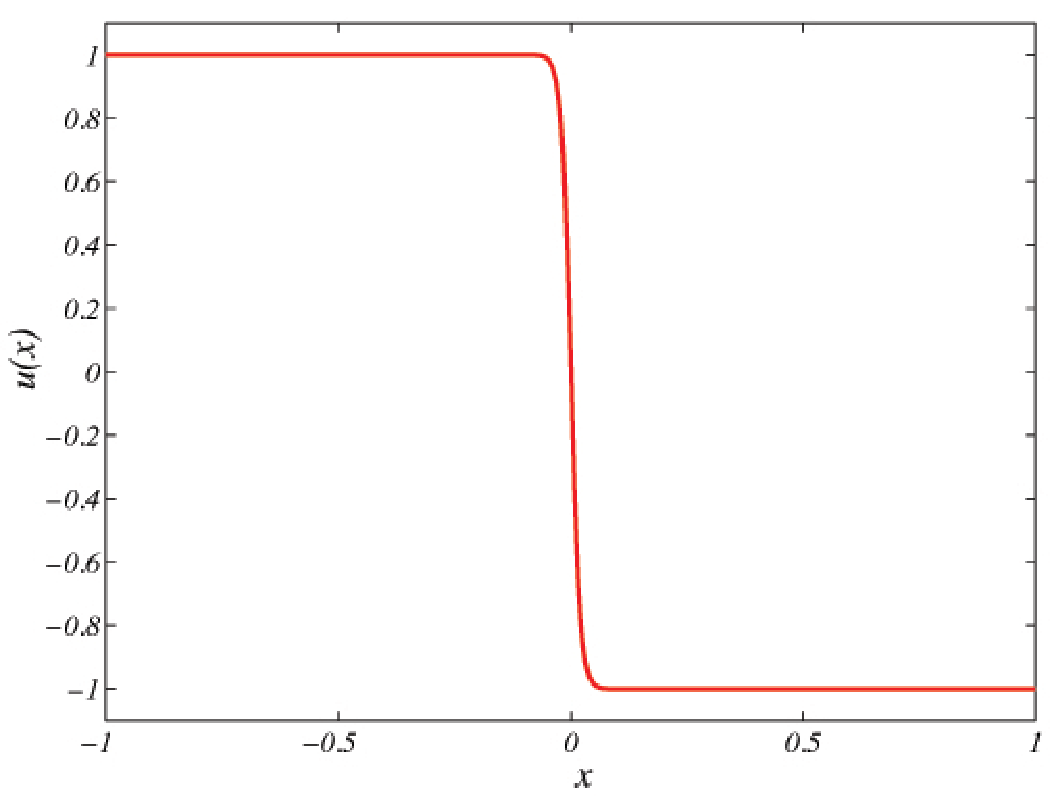
\includegraphics[width=4cm]{figures/SCALES_Presentations/Function.pdf}}
    \subfigure[Wavelet coefficient locations]{      \label{fig:DyadicGrid}
                                                    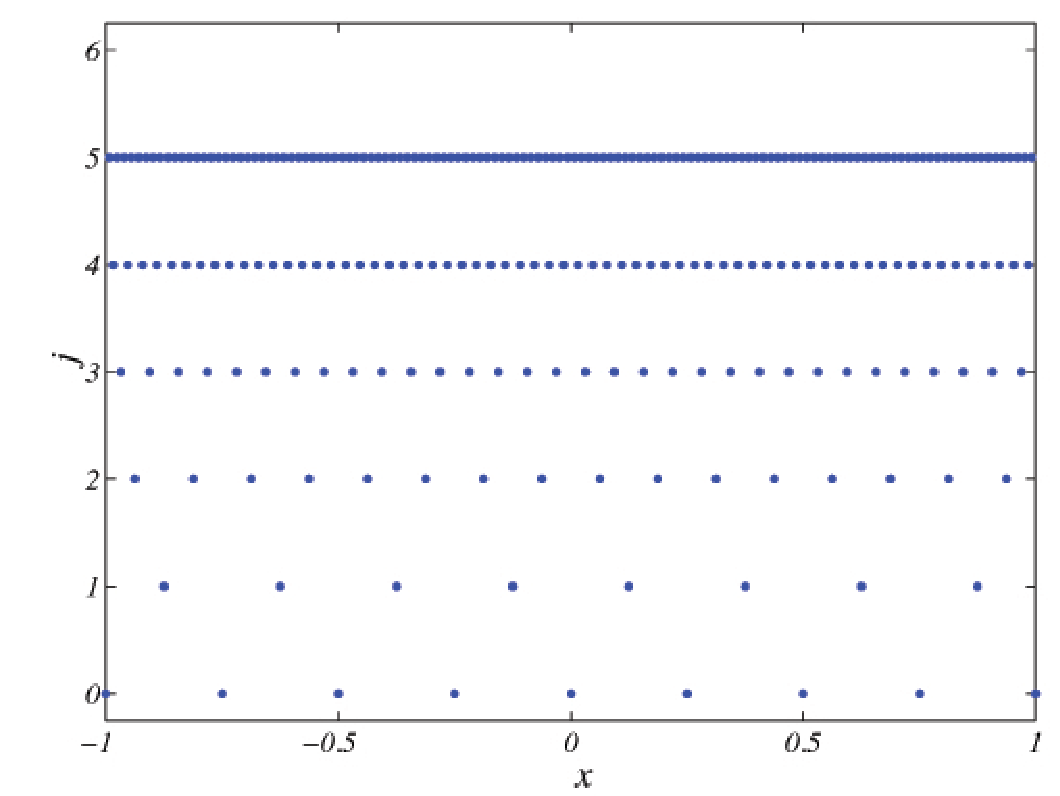
\includegraphics[width=4cm]{figures/SCALES_Presentations/wavelet_coefficient_locations.pdf}}
    \subfigure[Wavelet-threshold filter locations]{ \label{fig:WTFGrid}
                                                    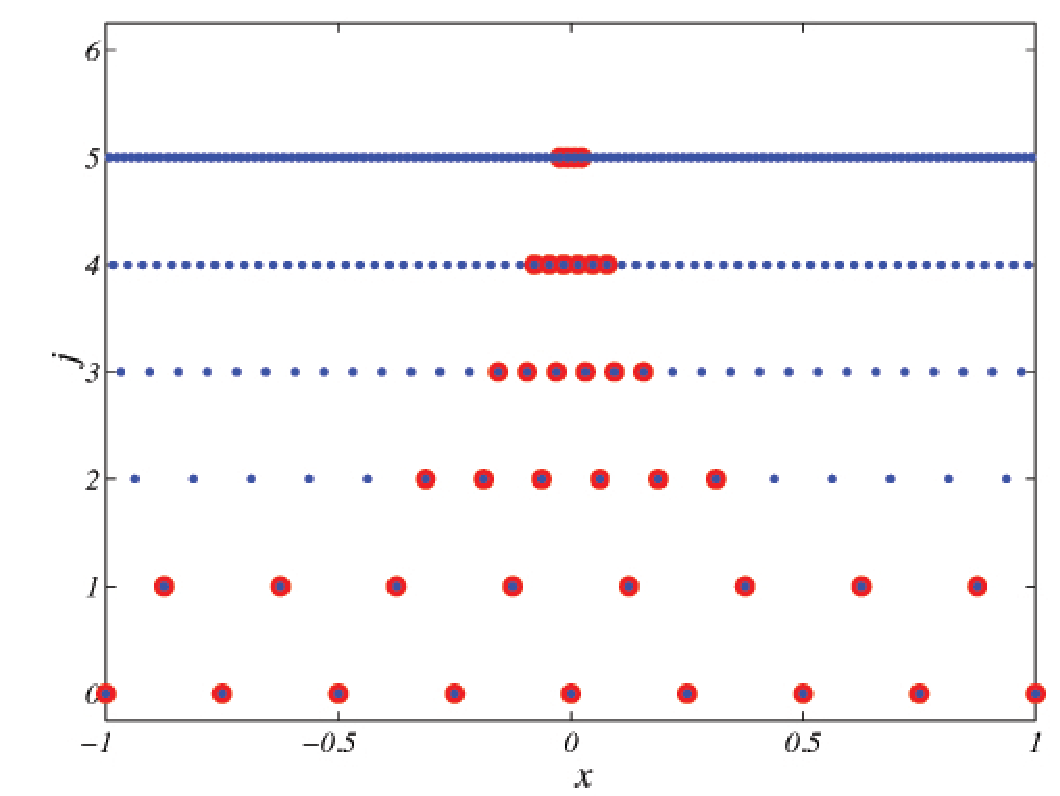
\includegraphics[width=4cm]{figures/SCALES_Presentations/wavelet_threshold_coefficient_locations.pdf}}
  \end{center}
  \caption{Schematic of Wavelet Threshold Filter}
  \label{fig:WTF}
\end{figure}



\begin{figure}[htp]
  \begin{center}
    \subfigure[Fourier Cutoff Filter]{     \label{fig:DNS_Fourier}
                                           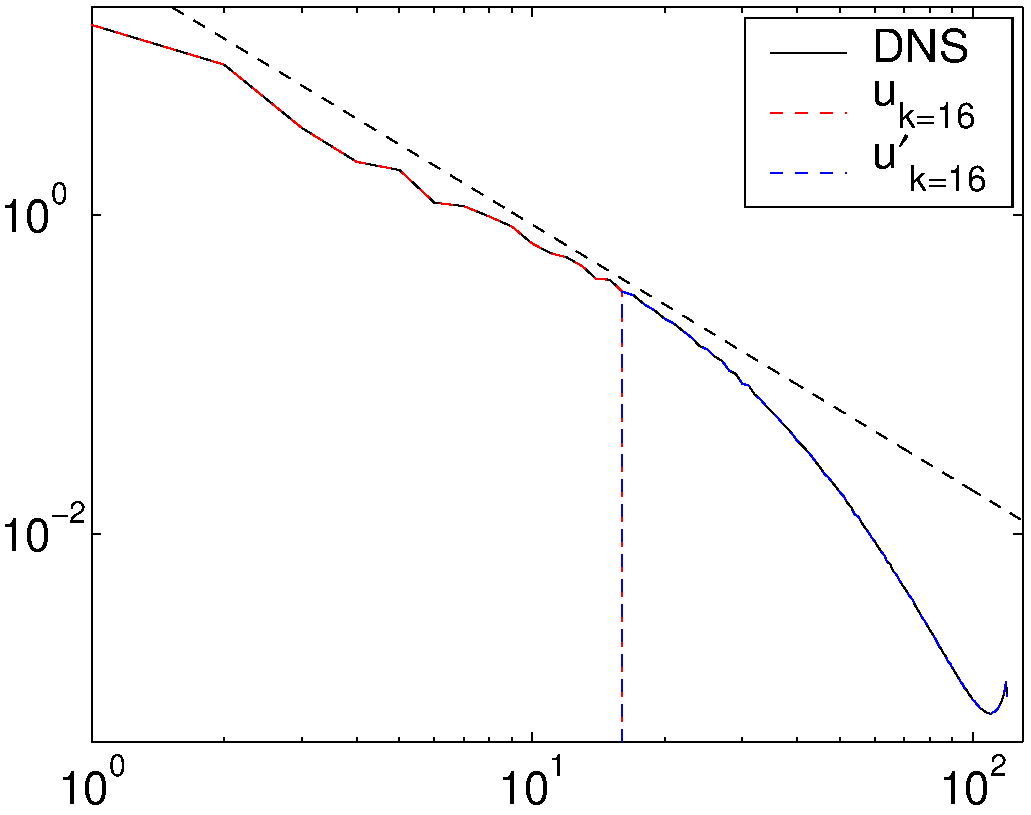
\includegraphics[width=5cm]{figures/SCALES_Presentations/f256_11_tst010_LI3M8JLEV5_fc_filt_kc16_spec.pdf}}
    \subfigure[Wavelet Threshold Filter]{  \label{fig:DNS_WTF}
                                           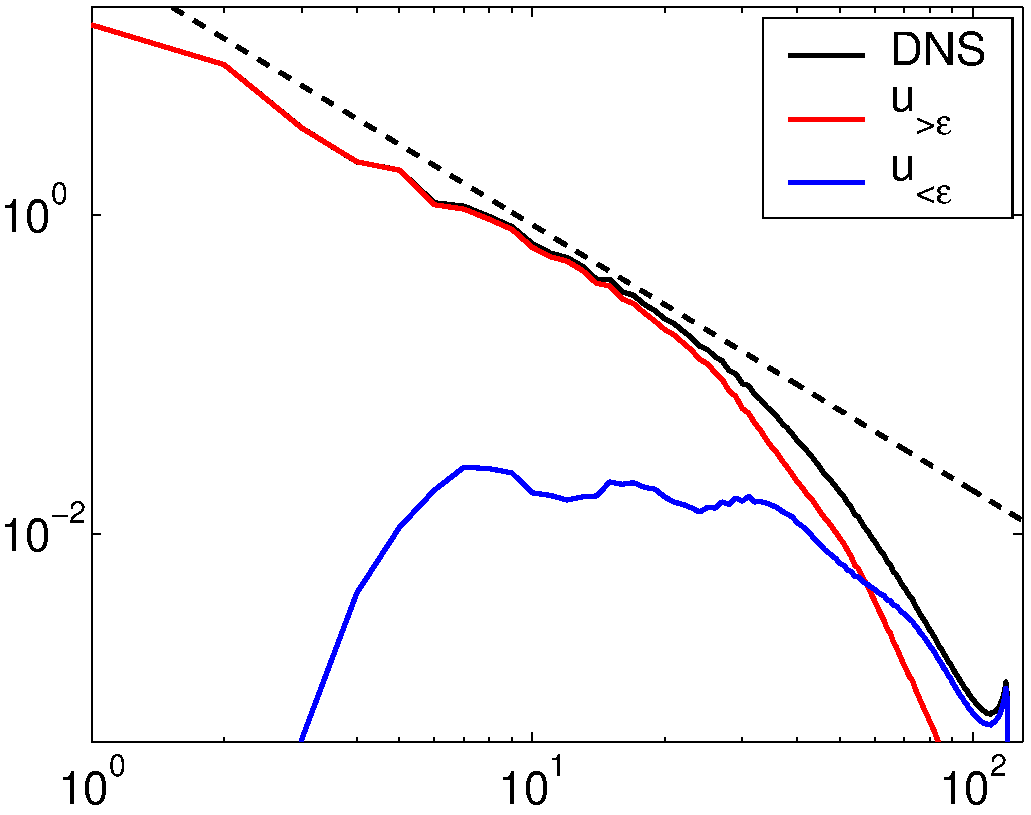
\includegraphics[width=5cm]{figures/SCALES_Presentations/f256_11_tst010_LI3M8JLEV5_wlt_filt_98_spec.pdf}}
  \end{center}
  \caption{Filtered DNS data on $256^3$ grid at $Re_{\lambda}\approx168$ }
  \label{fig:DNS_Filter}
\end{figure}



\begin{figure}[t]
\centerline{
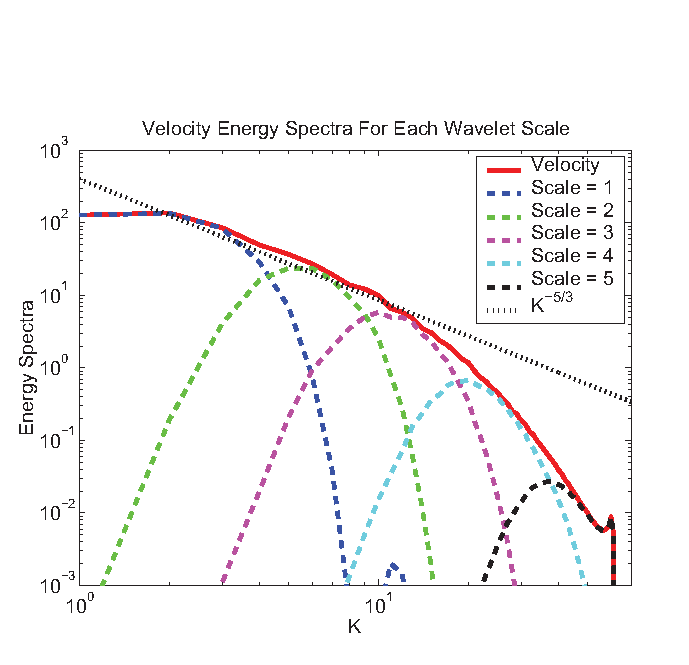
\includegraphics[width=8cm]{figures/SCALES_Presentations/WaveletScales_Levels.pdf}}
\caption{Velocity Energy Spectra For Each Wavelet Scale.}
\label{fig:WaveletScalesLevels}
\end{figure}


The astonishing wavenumber compression due to use of wavelets is evident in
a very insightful and artistic illustration, Fig.~\ref{fig:FargeSchneider_2001}, from a work by Farge and Schneider \cite{FTC_FargeSchneider_2001}
which showed that by transforming the vorticity field into wavelet space,
it can be realized that the high-concentration of active-wavelets are appeared only at few spatial locations.


%\begin{figure}[t]
%\begin{center}
%  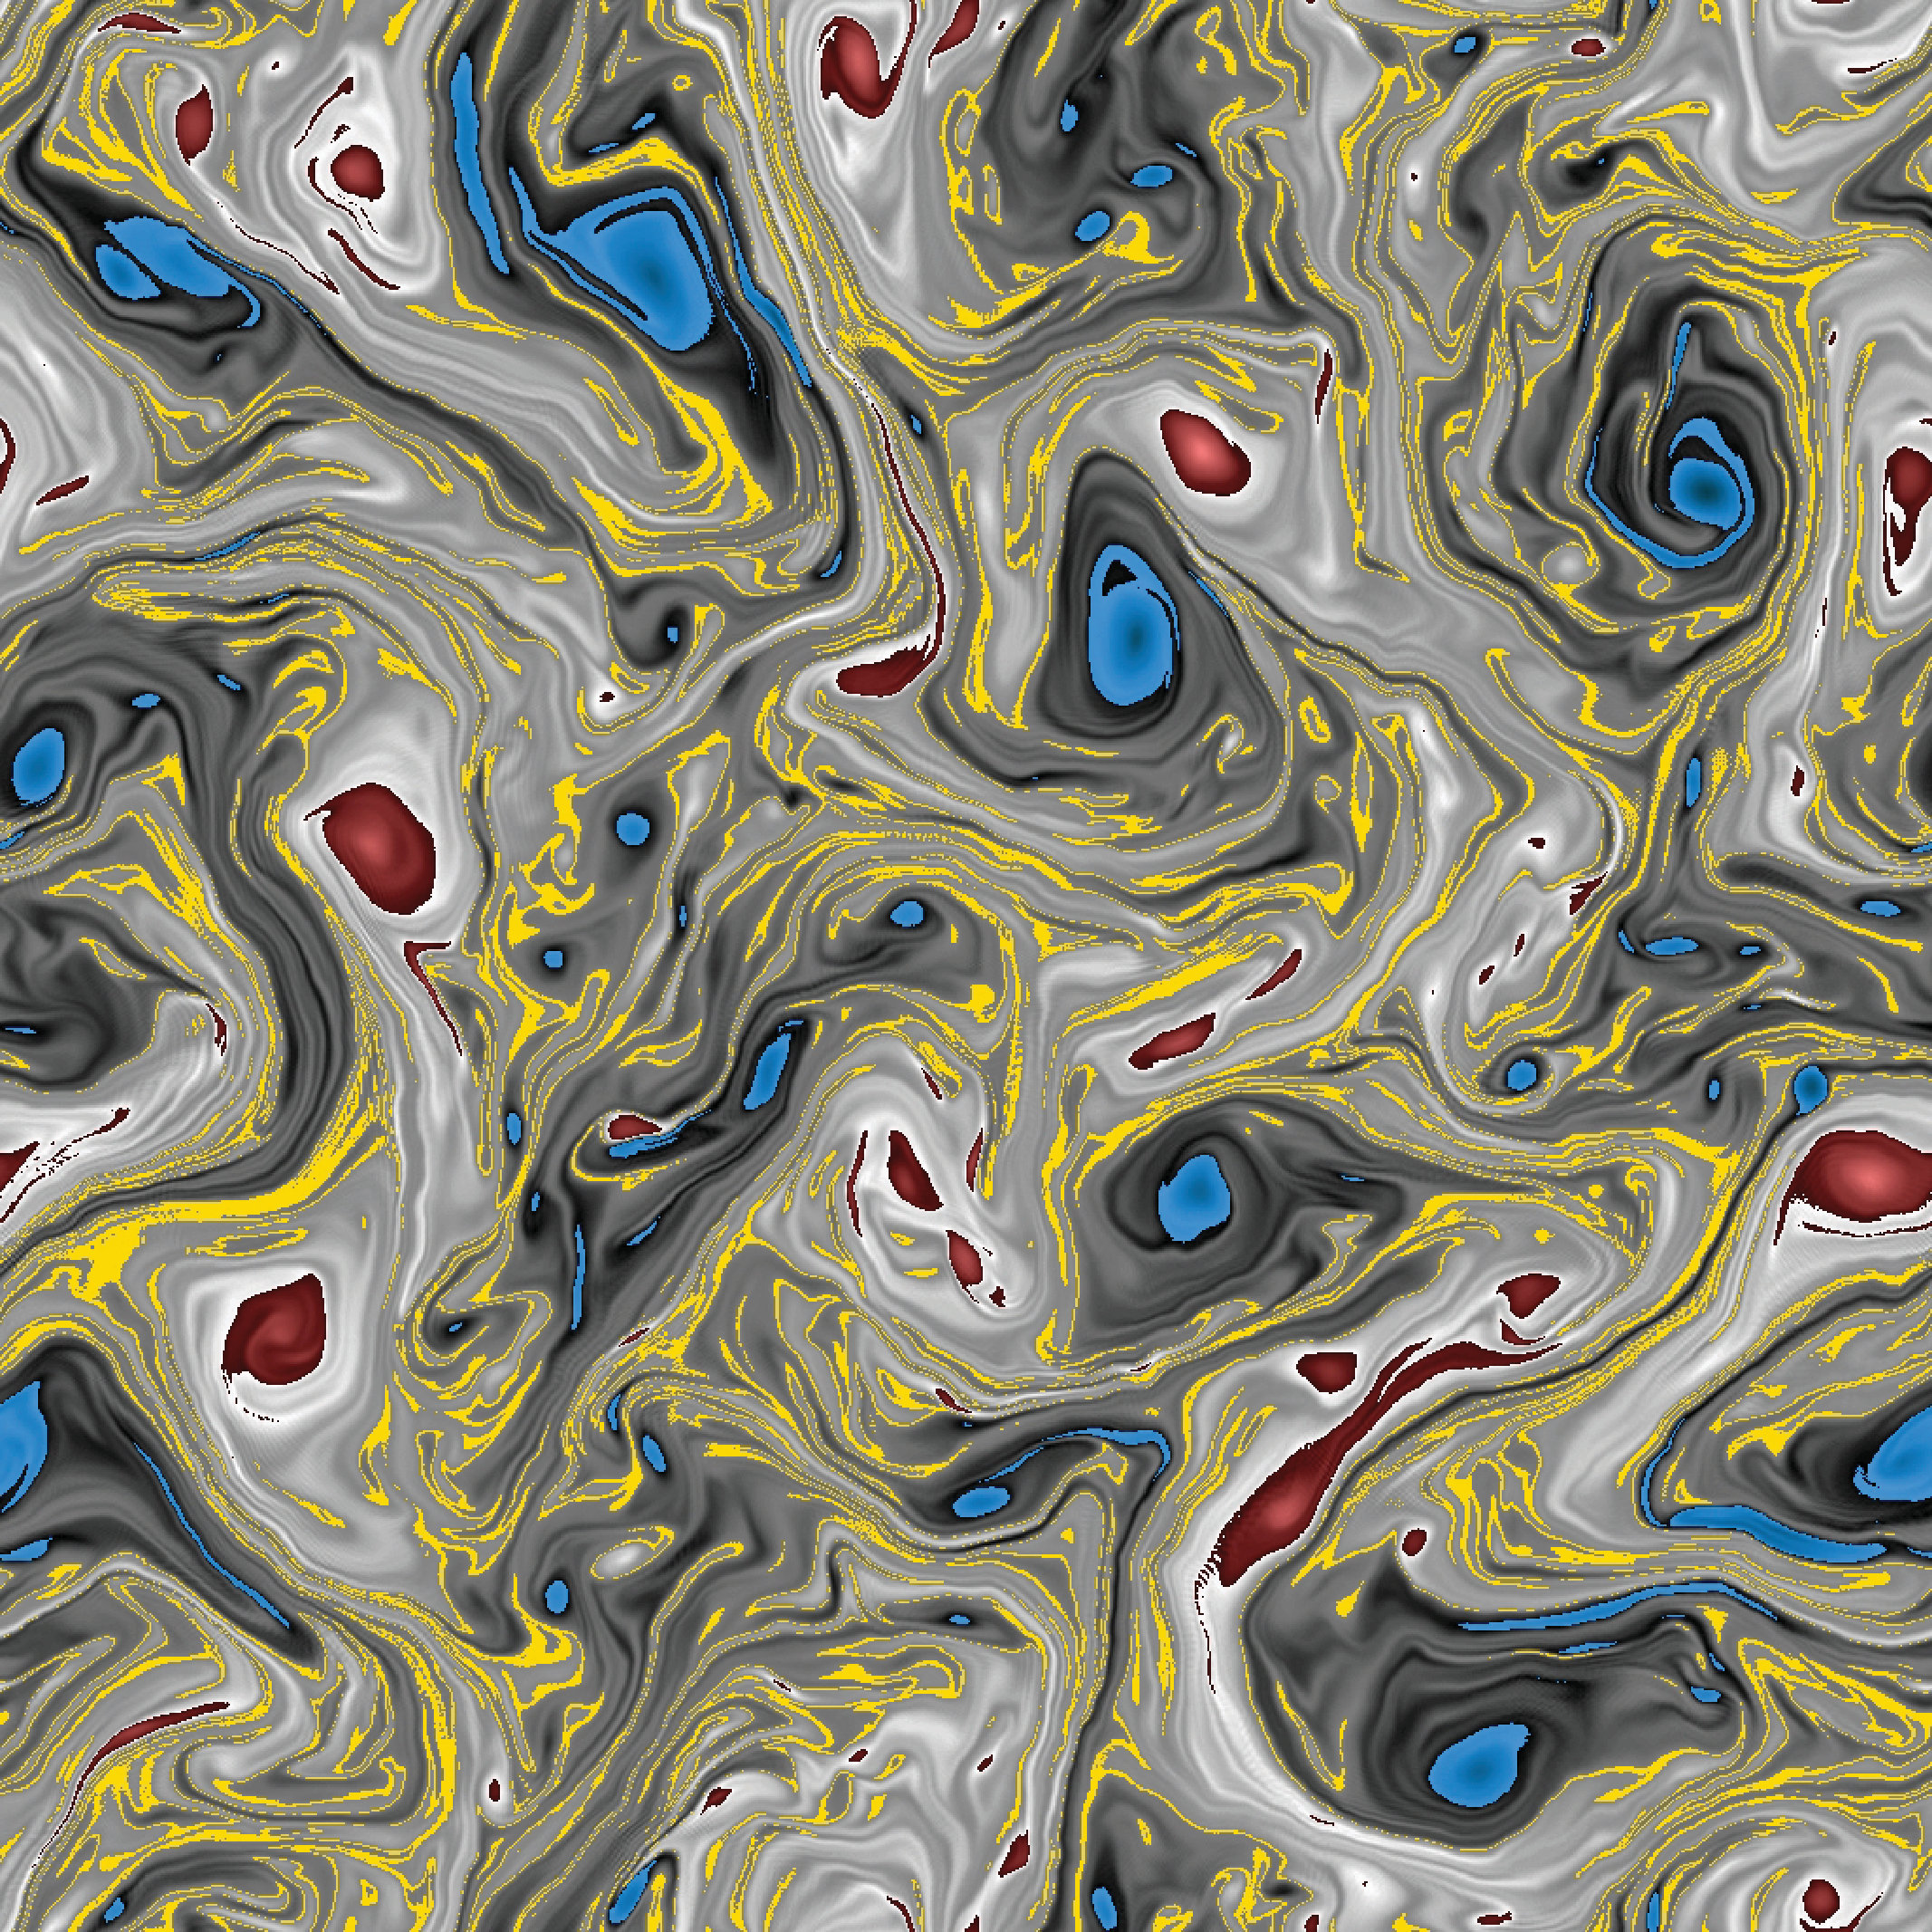
\includegraphics[width=0.5\textwidth]{figures/Farge_Schneider/vorticity.pdf}
%  %1in 4.5in 6.5in 10in
%  \caption{Wavelet transform of the Vorticity field: (a) Vorticity, (b) Active wavelet locations
%           Courtesy of Marie Farge and Kai Schneider  \cite{FTC_FargeSchneider_2001} }
%  \label{fig:FargeSchneider_2001}
%\end{center}
%\end{figure}



%\begin{figure}[t]
%\begin{center}
%\setlength{\unitlength}{0.01\textwidth}
%\begin{picture}(100,30)
%\put(-5,-3.5){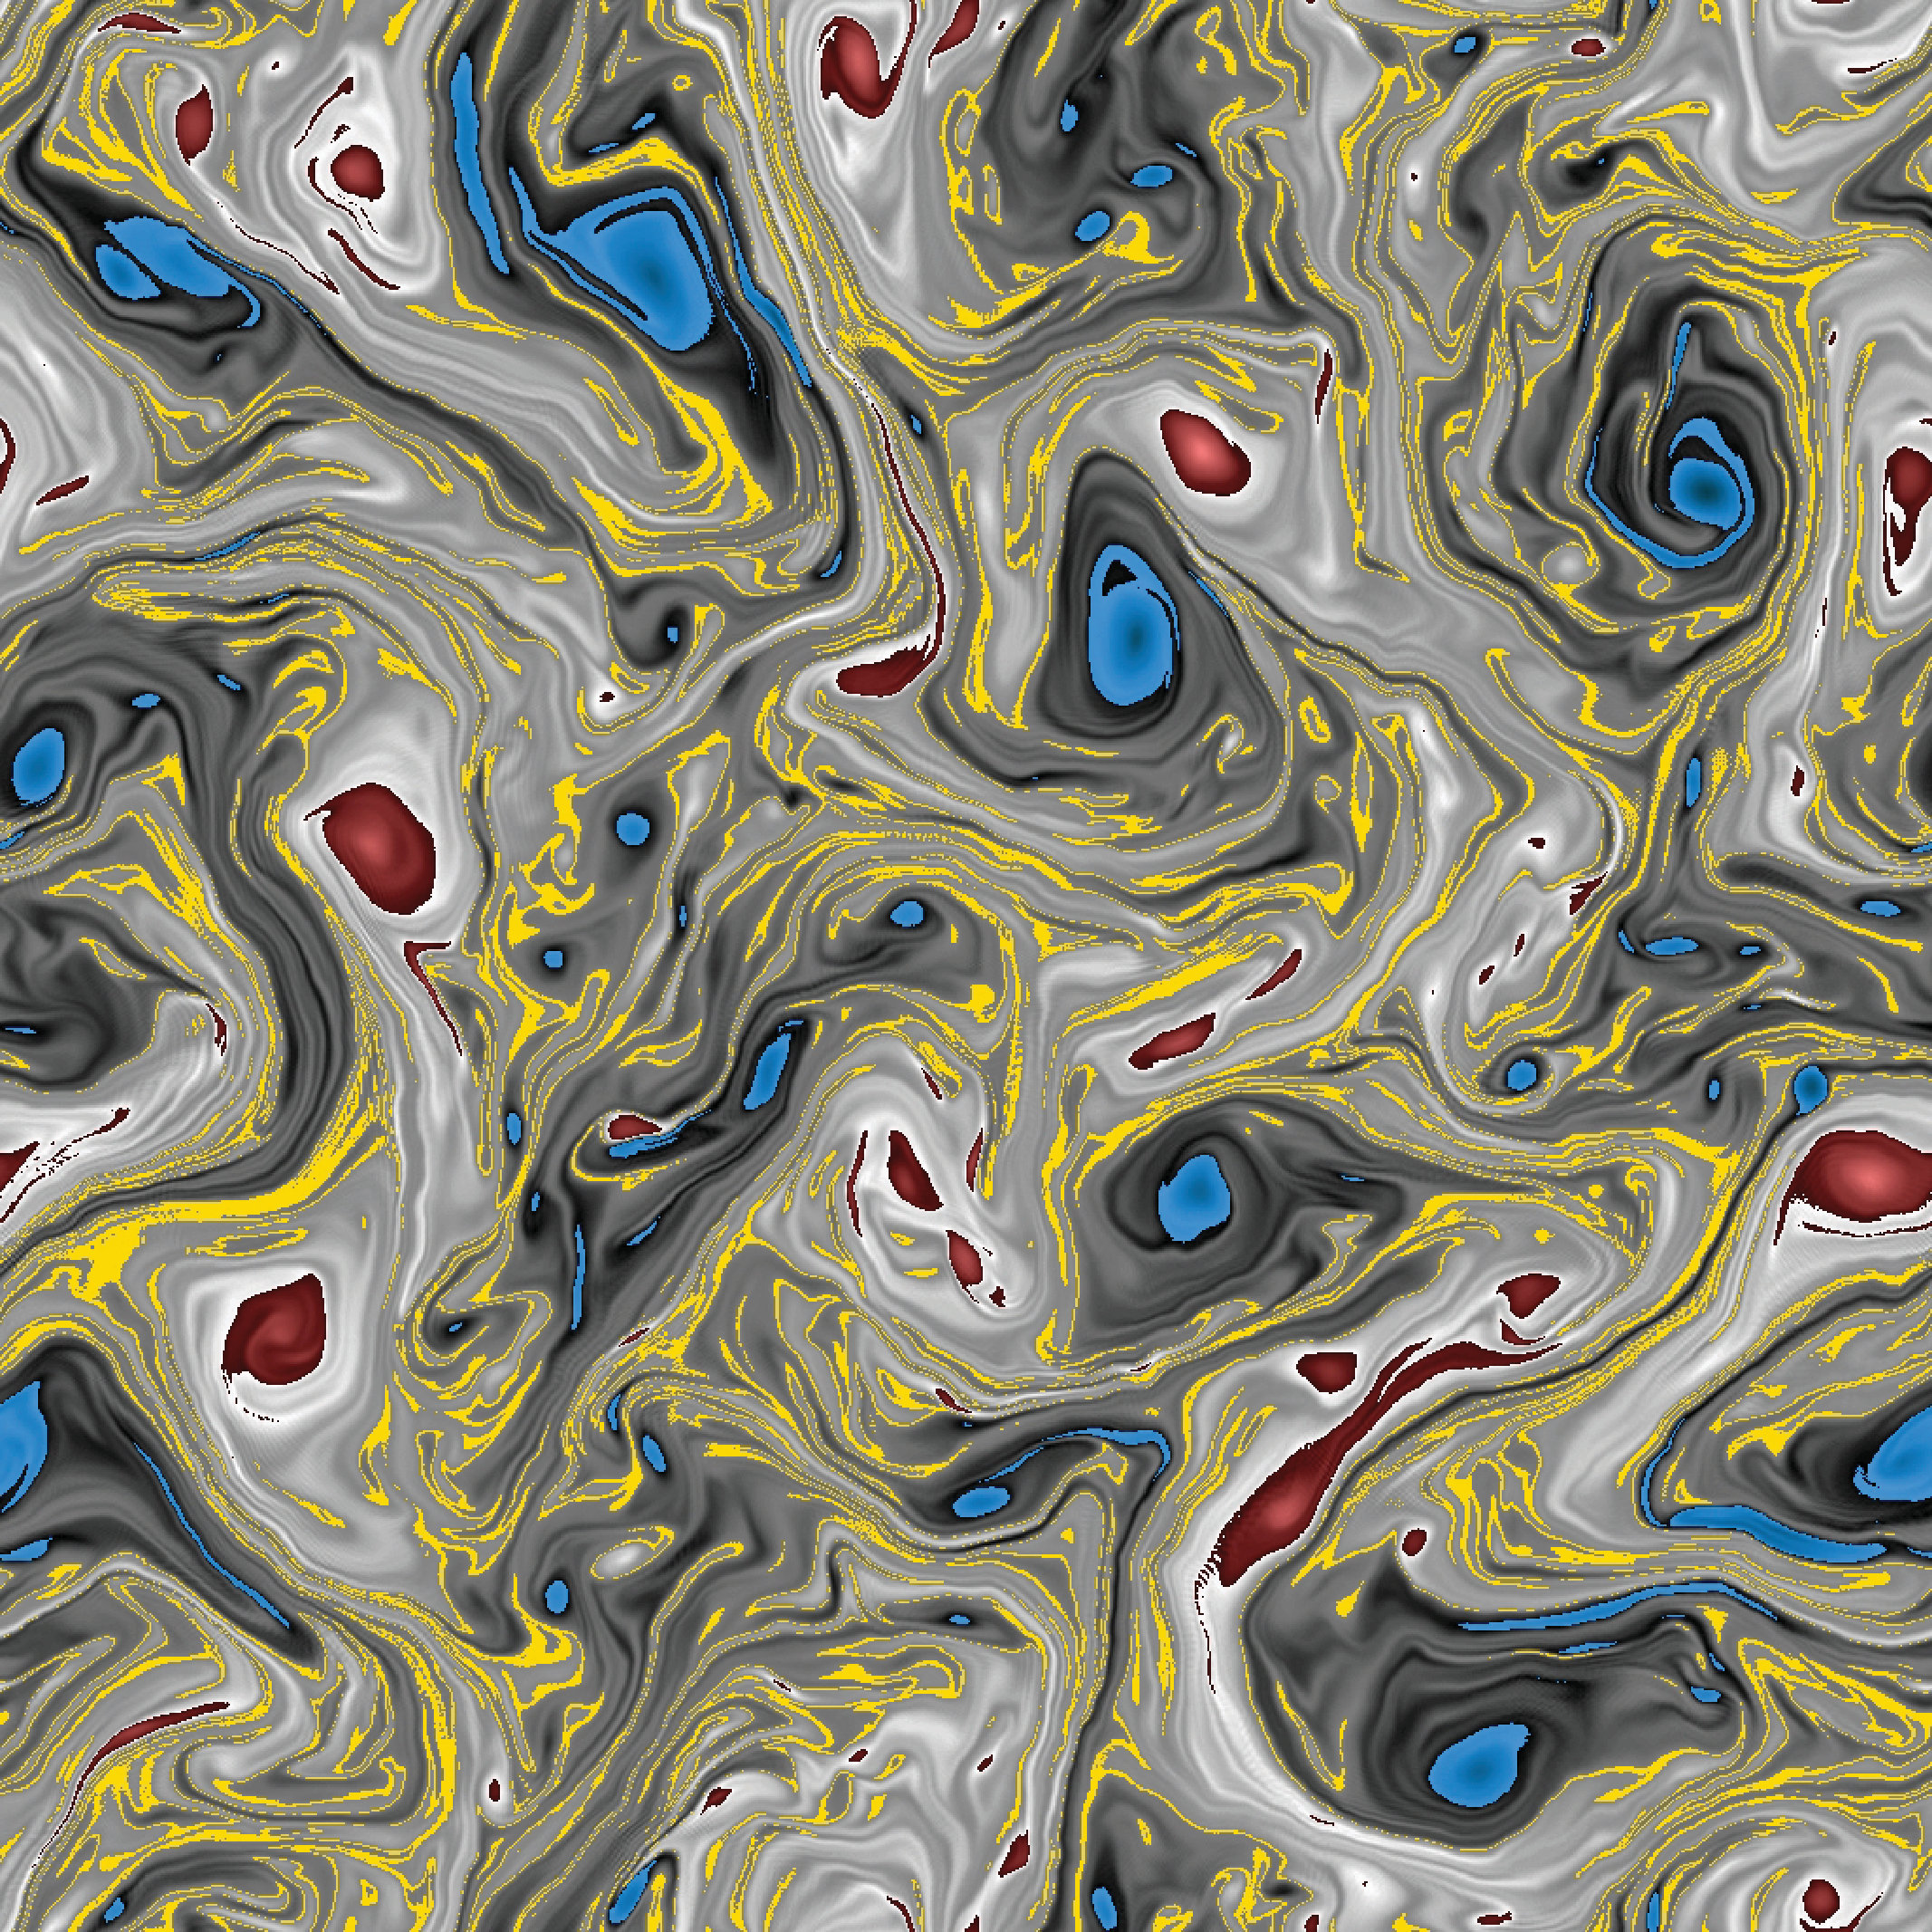
\includegraphics[height=0.34\textwidth]{figures/Farge_Schneider/vorticity.pdf}}
%\put(56,-3.5){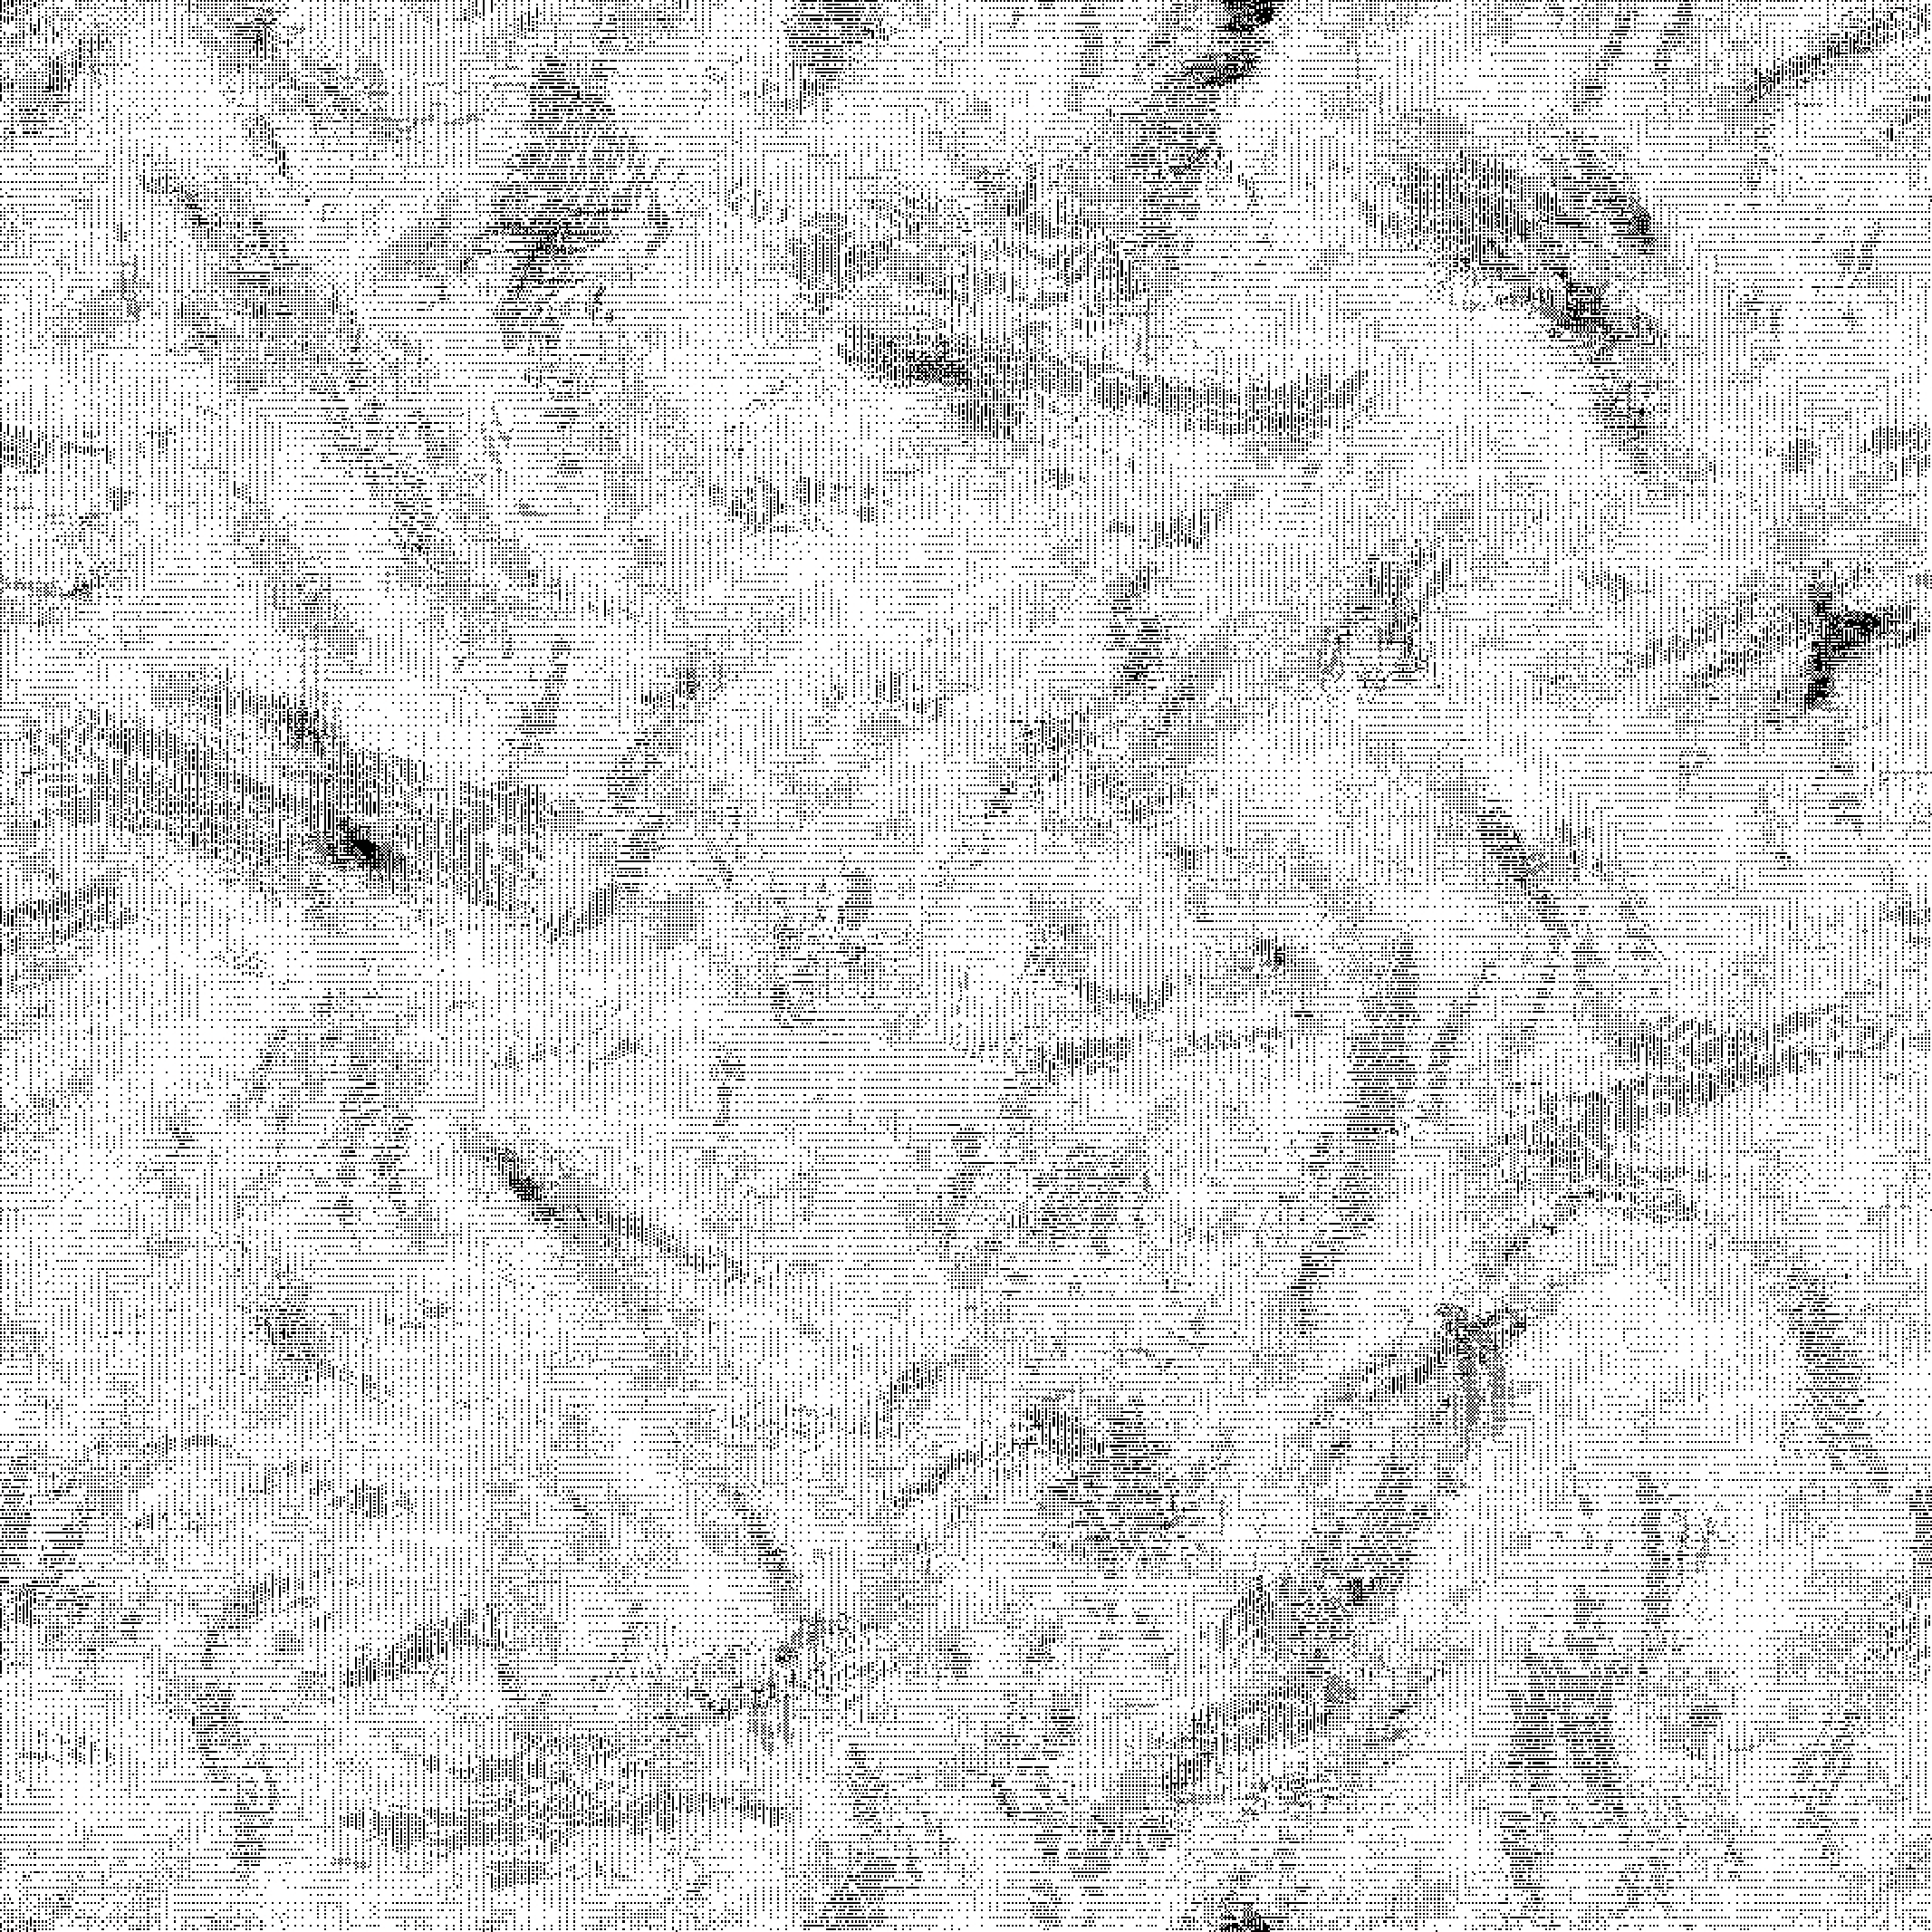
\includegraphics[height=0.34\textwidth]{figures/Farge_Schneider/ActiveWaveletLocations.pdf}}
%\put(4.5,25){(a)} \put(63,25){(b)}
%\end{picture}
%\end{center}
%\caption{Wavelet transform of the Vorticity field: (a) Vorticity; (b) Active wavelet locations.
%           Courtesy of Marie Farge and Kai Schneider  \cite{FTC_FargeSchneider_2001}. }
%\label{fig:FargeSchneider_2001}
%\end{figure}

\begin{figure}[t]
  \begin{center}
    \subfigure[Vorticity]{                 \label{fig:FargeSchneider_2001_Vorticity}
                                           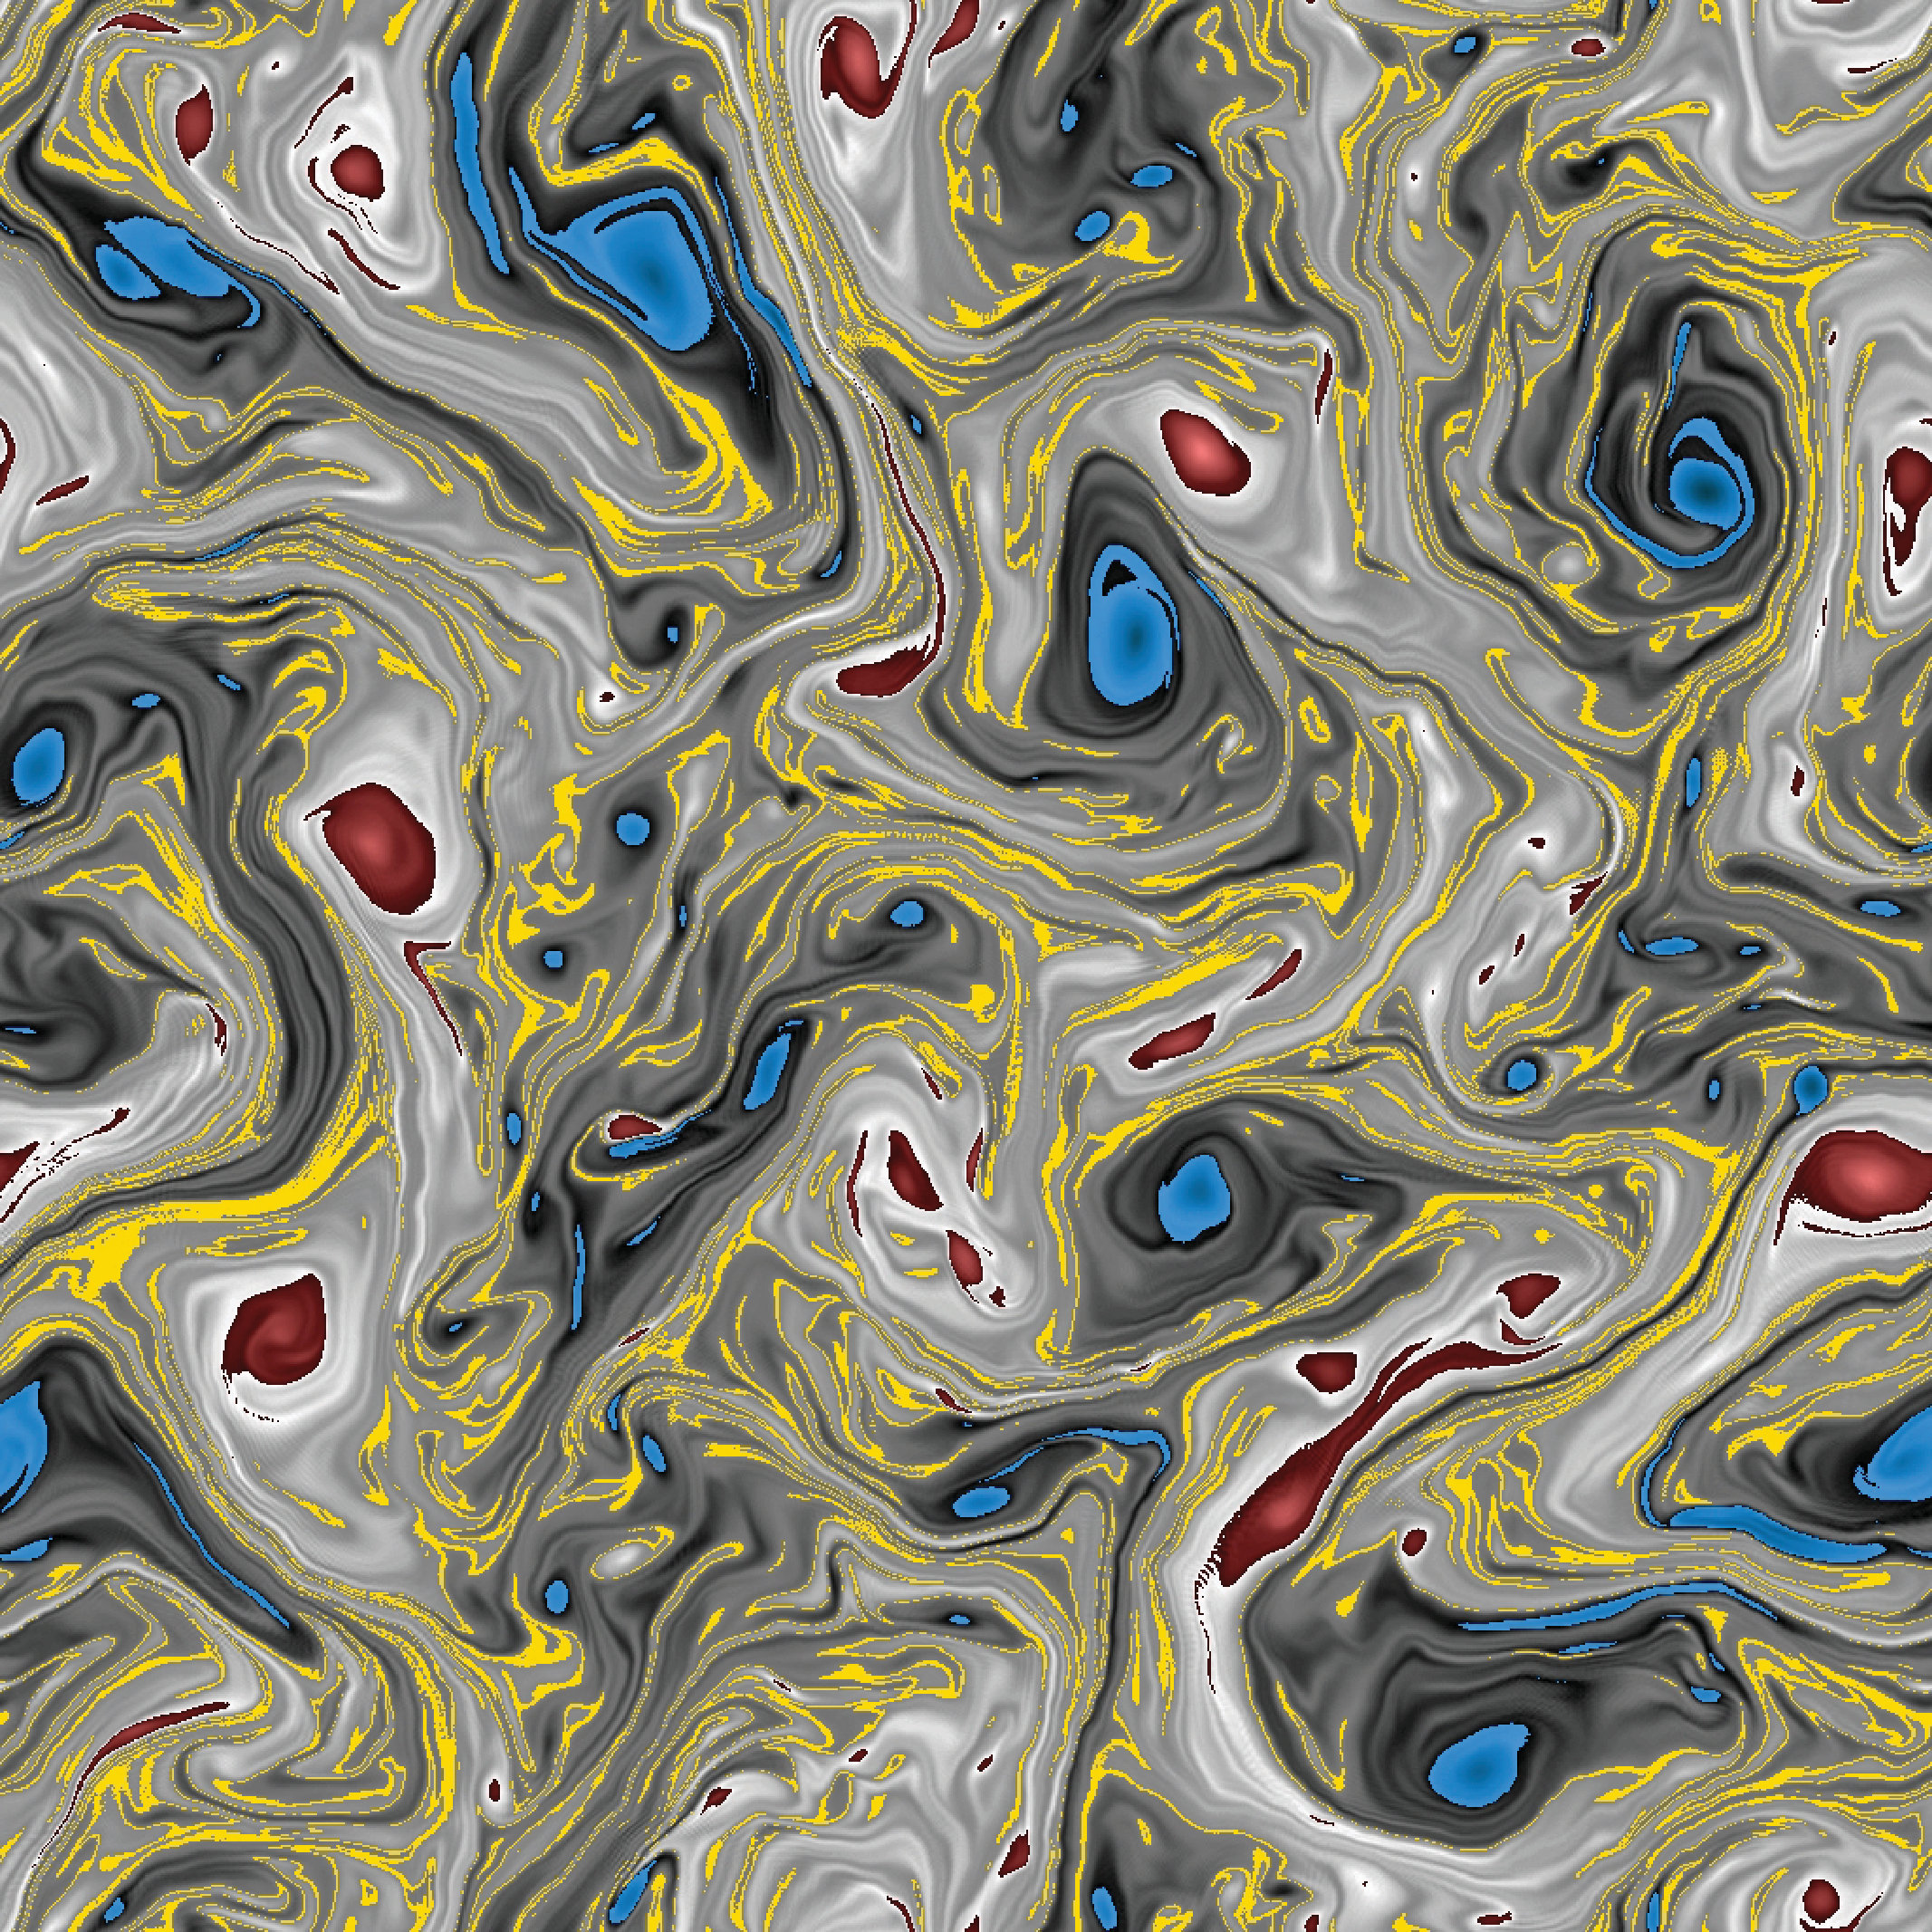
\includegraphics[width=6cm]{figures/Farge_Schneider/vorticity.pdf}}
    \subfigure[Active wavelet locations]{  \label{fig:FargeSchneider_2001_ActiveWavelets}
                                           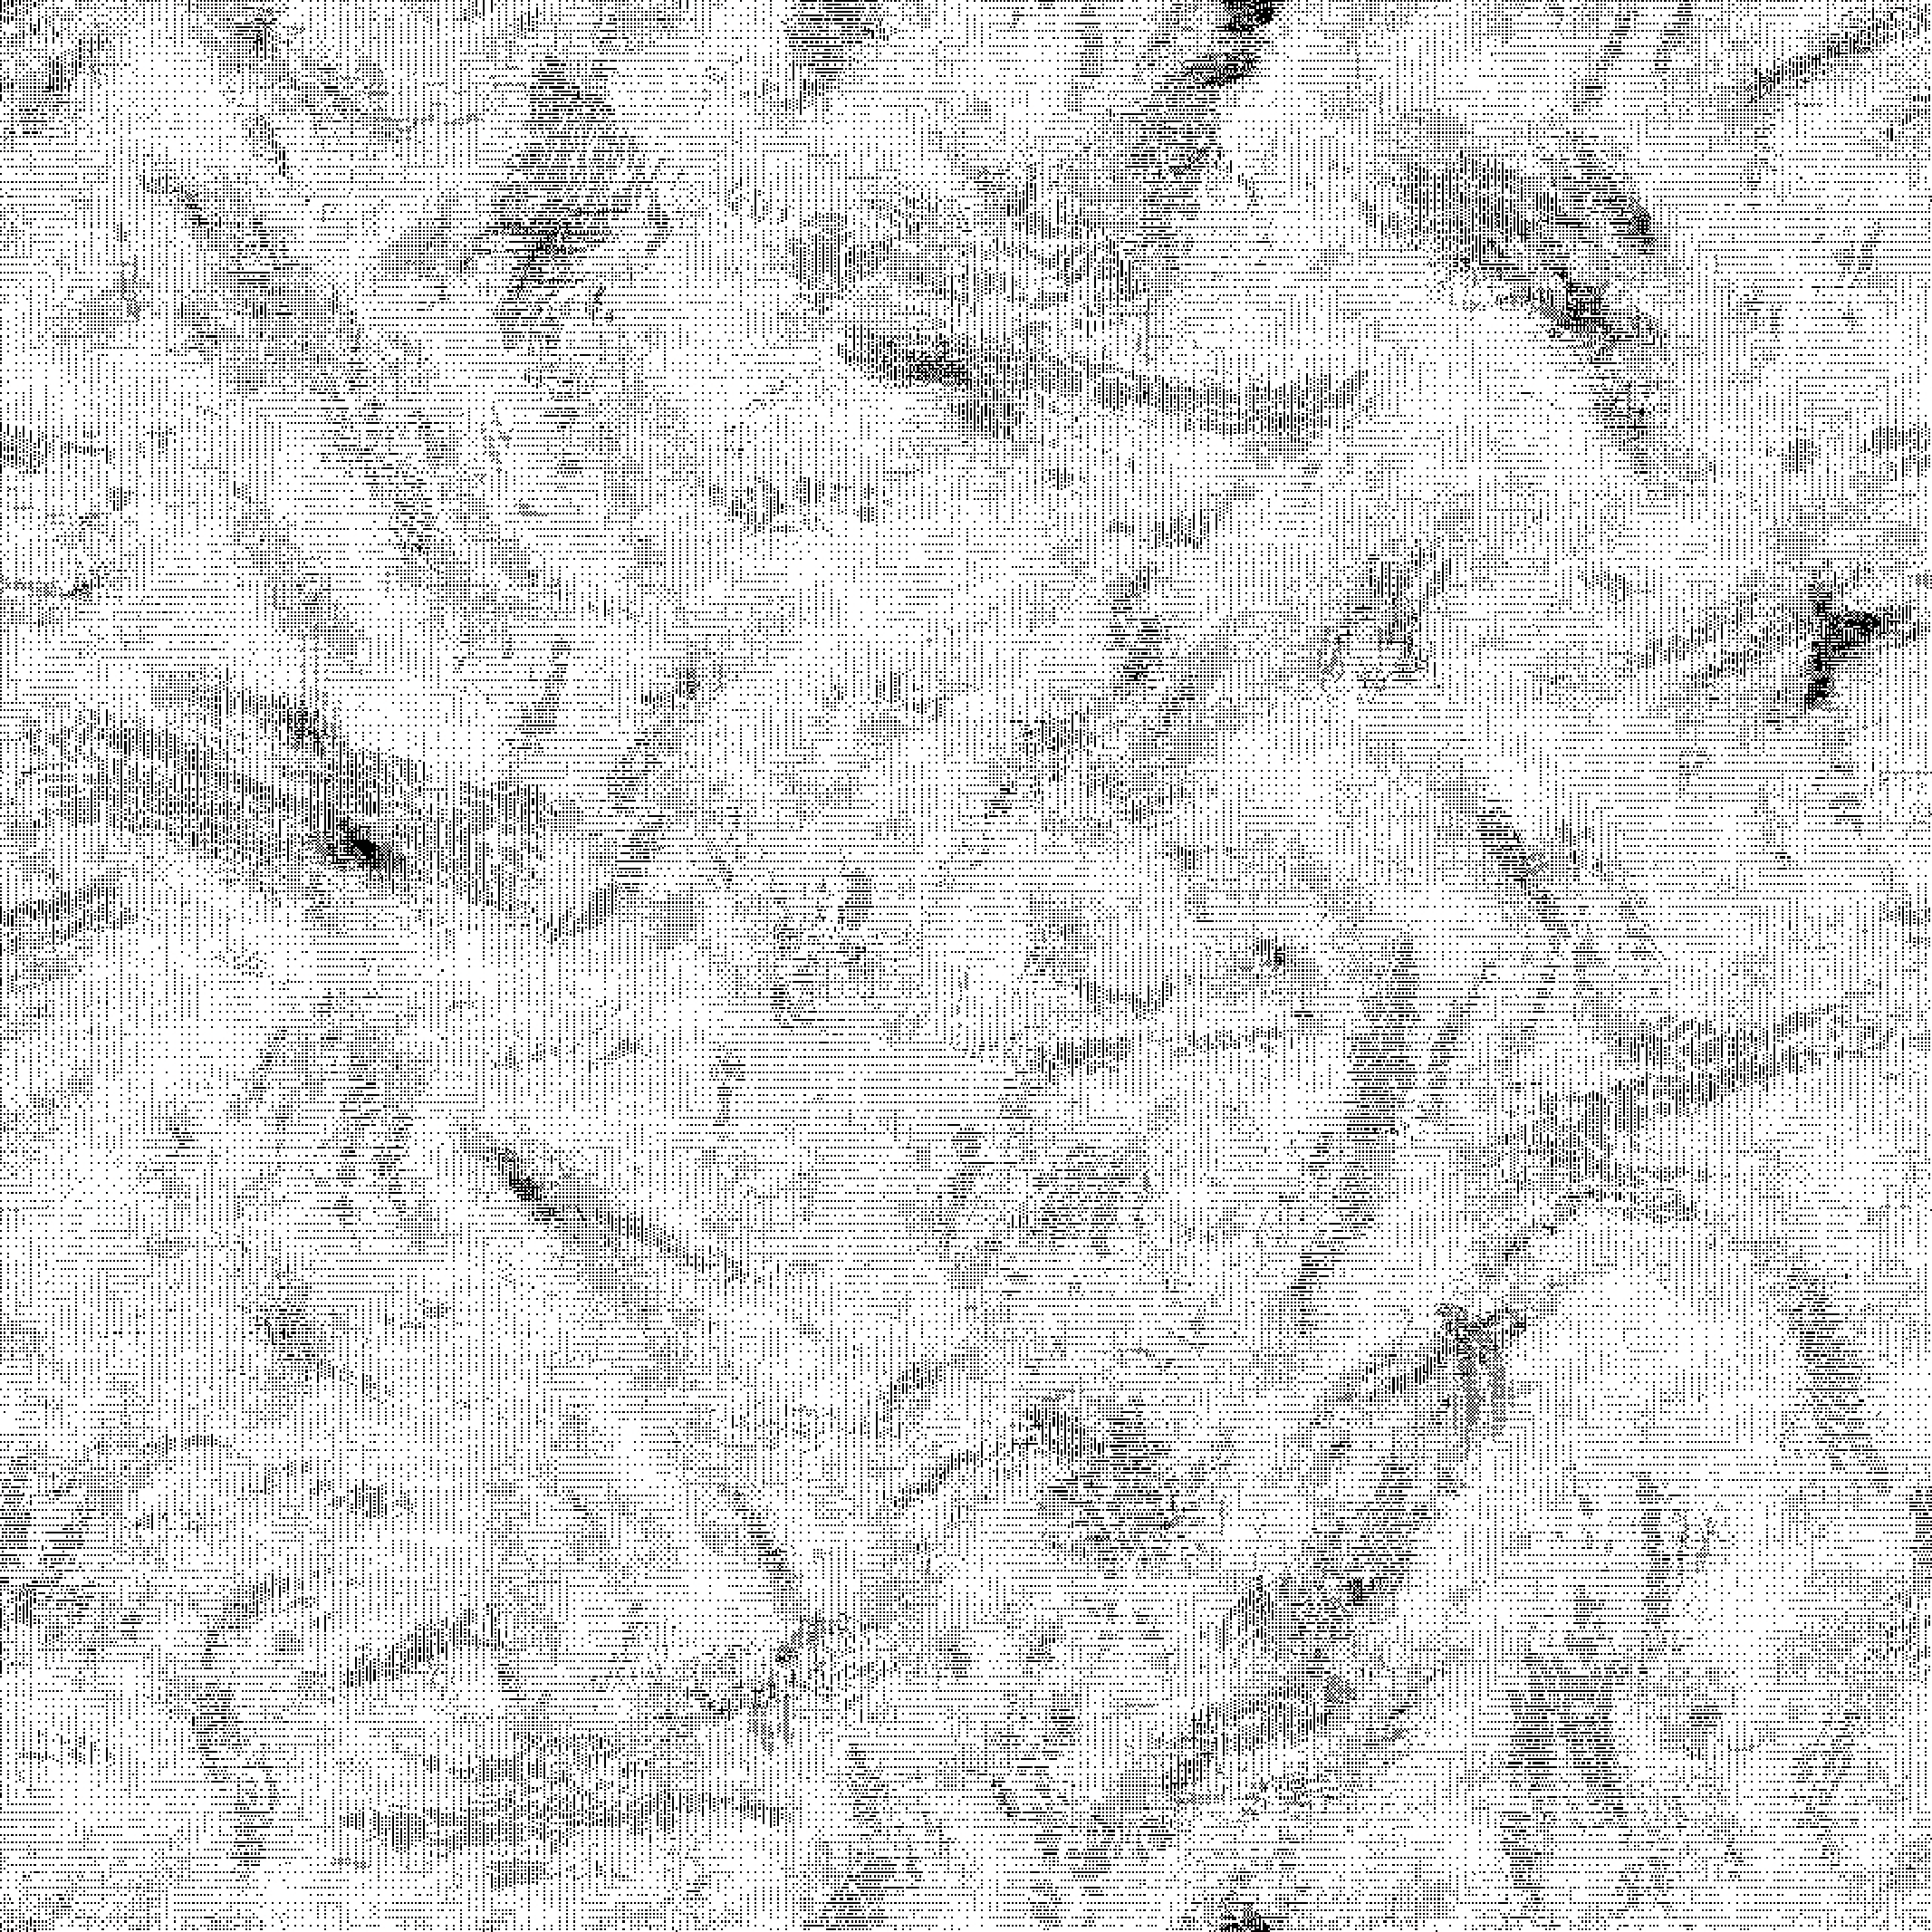
\includegraphics[width=6cm]{figures/Farge_Schneider/ActiveWaveletLocations.pdf}}
  \end{center}
  \caption{Wavelet transform of the Vorticity field. Courtesy of Marie Farge and Kai Schneider  \cite{FTC_FargeSchneider_2001}. }
  \label{fig:FargeSchneider_2001}
\end{figure}






%%?????????????????????????????????????????
%%\parbox[t][0.4cm]{16cm}{
%%\parbox[t][0.2cm]{7cm}{
%%\marginpar{
%\setlength{\marginparwidth}{2cm}
%\marginpar{\raggedleft \tiny  %\footnotesize  %\raggedright
%\textcolor[rgb]{0.64,0.28,1.00}{
%%\footnotesize{ \\ \\
%$\clubsuit$
%If I mention WURANS and CVE, I have to write about them.
%Though, I am not sure if it ie necessary to talk about them.
%On the other hand, if I don't mention them here, then I will miss 2 categories ?!!
%}}
%%?????????????????????????????????????????





The wavelet based methods mainly categorized into WDNS (Wavelet based DNS), CVS (Coherent Vortex Simulation), and SCALES(Stochastic Coherent Adaptive Large Eddy Simulation).



%%%%%%%%%%     W  D  N  S     %%%%%%%%%%%%%%%%%%%%%%%%%%%%%%%%%%%%%%%%%%%%%%%%%%
WDNS -- proposed for the first time by Fr\"{o}hlich and Schneider \cite{WDNS_1996} -- is in fact and Adaptive-DNS where the wavelet-based numerical methods used to solve Navier-Stokes equations without any model
with a sufficiently small threshold in order to ensure that the ignored-scales are not significant.
As a result of wavelet filtering and due to compression property of wavelets, the number of DOF (degree-of-freedom) reduced compared with DNS;
however, still due to small threshold, it is very expensive or better to say impossible for real flow applications:
the 2D spatial computational complexity scales as $Re^{\frac 1 2}$.





%%%%%%%%%%     C  V  S     %%%%%%%%%%%%%%%%%%%%%%%%%%%%%%%%%%%%%%%%%%%%%%%%%%
CVS -- proposed by Farge et al. \cite{CVS_POF_1999} -- is based on the idea that coherent modes are the ones which are mostly responsible for the evolution of the turbulence and the fully developed turbulence is made of: 1) an organized coherent part; and 2) a random incoherent part.
%
It was observed that by filtering the vorticiy field using orthogonal wavelet bases, the probability density function (PDF) of the unresolved filed is of the form of PDF of Gaussian white noise. Therefore, CVS (wavelet-filtered vorticity with an optimal threshold) is an approach to decompose the flow into deterministic and stochastic fields.
%
Therefore, in CVS 1) the coherent-structures (the wavelet de-noised vorticity-field) are simulated directly; and
2) The incoherent-structures is considered as a Gaussian white noise:
(``resulting SGS field''  by CVS  is  ``near Gaussian white noise'') that provides no turbulent-dissipation.





%%%%%%%%%%     S  C  A  L  E  S     %%%%%%%%%%%%%%%%%%%%%%%%%%%%%%%%%%%%%%%%%%%%%%%%%%

%The properties of wavelet transform, namely  the ability to identify and efficiently represent temporal/spatial coherent flow structures,  self-adaptiveness, and \linebreak[4] de-noising, have made them attractive
%candidates for constructing multi-resolution variable fidelity schemes  for simulations of turbulence \cite{ARFM_2010}.
Stochastic Coherent Adaptive Large Eddy Simulation (SCALES) \cite{POF_2004}
is a recent wavelet-based methodology for numerical simulations
of turbulent flows that resolves energy containing turbulent motions using
wavelet multi-resolution decomposition and self-adaptivity. In this technique, the extraction of
the most energetic structures is achieved using wavelet thresholding filter
with a priori prescribed threshold level.

%The major motivations of SCALES can be summarized as:
% 1) separation of most- and less-energetic structures (unlike large- and small-structures in LES, or coherent and incoherent structures in CVS);
% 2) grid adaptation based on instantaneous flow realization;
% 3) making SGS model adaptive based on the filter thresholding-factor and spatial-varying filter width (unlike fixed filter width in LES) and consequently SGS terms benefited from wavelet nonlinear multiscale band-pass filter which depends on instantaneous flow realization (unlike linear low-pass filters in classical LES);
% 4) not limited to fully developed turbulence because of the assumption of negligible turbulent-dissipation (unlike CVS);
% 5) having local SGS models.

SCALES is a methodology, which inherits the advantages of both Coherent Vortex Simulations (CVS) \cite{CVS_POF_1999} and Large Eddy Simulation (LES) while overcoming the shortcomings of both.
Unlike coherent/incoherent and large/small structures decomposition in CVS and LES respectively,
in SCALES the separation is between more and less energetic structures.
Therefore, unlike CVS, the effect of background flow can not be ignored and needs to be modeled similarly to LES.
Furthermore, the filtering and consequently,the subgrid scale (SGS) model are benefited from
wavelet nonlinear multiscale band-pass filter, which depends on instantaneous flow realization.
As a result of using SGS models, the number of degrees-of-freedom is smaller than CVS and consequently a higher grid-compression can be achieved.

In SCALES, the Navier-Stokes equations are solved using the adaptive wavelet collocation method (AWCM) \cite{JCP_2000}
which is based on the second-generation bi-orthogonal wavelet -- a compactly supported and symmetric scheme.

Unlike the CVS which is based on vorticity equations, SCALES similar to LES solves the velocity field and it was proved that using
bi-orthogonal wavelets, the PDF of the modeled portion of the SGS (wavelet-filtered out) velocity field is of the form of Gaussian white noise PDF.

This fraction of the less energetic structures is in fact a small part of SGS field.
That is to say, the velocity field is initially decomposed to more and less energetic structures by means of wavelet-threshold filter.
The ``deterministic most energetic coherent structures'' are solved directly using AWCM. However, the unresolved field in not absolutely an incoherent stochastic field with no effect on the resolved field and as a result, it needs to be modeled. Again, using wavelet-threshold filter, the
unresolved field is decomposed into two kinds of modes:
the minority ``deterministic coherent SGS modes''; and the ``majority stochastic incoherent SGS modes''.
The effect of these two modes on the resolved field  can be modeled by ``deterministic SGS models'' and ``stochastic SGS models'' respectively.

%Main Differences with CVS/LES Separation between resolved-coherent-structures and unresolved-eddies is now
%Separation between range-of-more-energetic-eddies       Effect of Background flow in not negligible and must be models (SGS models)
%L1)  So similar to LES   BUT   benefited from wavelet nonlinear multiscale band-pass filter
%                                               depends on instantaneous flow realization
%                                     NOT   linear low-pass filters (in classical LES)
%C2) No assumption of negligible turbulent-dissipation   associated to SGS structures
%       ( SGS models will approximate (model) them )
%       Therefore, NOT limited to  �Fully developed turbulence�
%C3)  Using SGS models                   reduce  DOF                       increase  Grid-Compression
%
%Even by less than %1 of total non-adaptive grid points, DNS matched results obtained
%
%To fully being benefited from Dynamic-Adaptability:  2 Local SGS models proposed
%   1)  Localized Dynamic Kinetic-Energy Based Model (LDKM)
%   2)  Lagrangian Dynamic SGS (LDM)

The overall at-a-glance comparison of these wavelet-based methods -- WDNS, CVS, SCALES -- and the non-wavelet-based methods -- DNS, LES --
can be easily illustrated in Coherency Diagram, Fig.~\ref{fig:CoherencyDiagram}, on which the wavenumber increase in the horizontal direction and the wavelet-threshold-filter threshold-parameter increase in the vertical direction upward. It is clearly shown that the CVS and LES are limiting case of Coherent/Incoherent and Large/Small structures distinctions while in SCALES in a more relaxed fashion, both resolved and unresolved structures are not limited to these separations. Therefore, while not being limited to homogenous-turbulence -- as is the case in CVS -- with a very high grid-compression ratio, majority of important energetic structures are resolved and both coherent-deterministic and incoherent-stochastic unresolved modes can be modeled. This distinction is not anymore limited to the size of the structures -- which is rather less informative -- as it is the case in classical LES. Furthermore, resolved structures and the modeled eddies share a range of wavenumbers together in order to ensure more realistic energy cascades.

\begin{figure}[t]
\begin{center}
  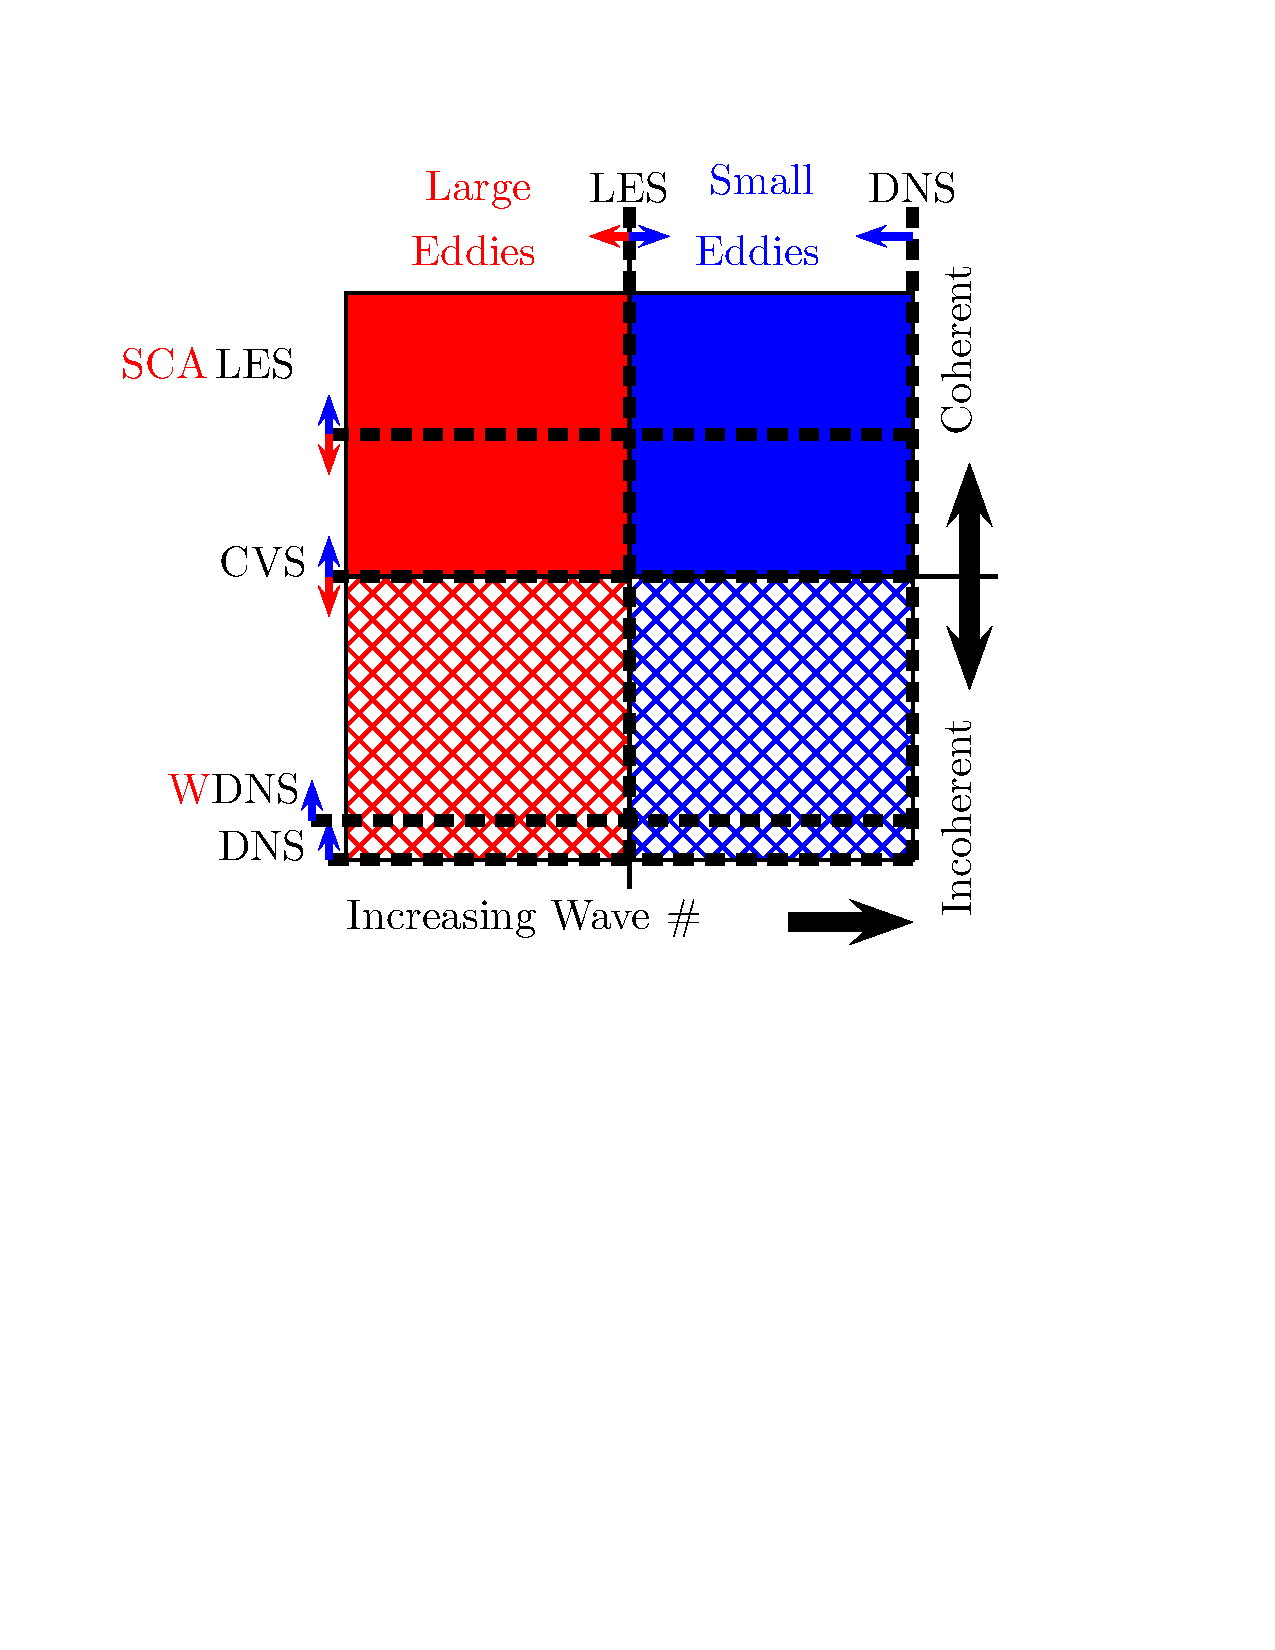
\includegraphics[clip=true, viewport=20mm 108mm 170mm 253mm, width=0.5\textwidth]{figures/SCALES_Presentations/diagram_1.pdf}
  %1in 4.5in 6.5in 10in
  \caption{Coherency Diagram: At-a-Glance Comparison of DNS, WDNS, CVS, SCALES, LES.}
  \label{fig:CoherencyDiagram}
\end{center}
\end{figure}










\section{Motivation}

Ever since the emergence of the wavelet-based multi-resolution schemes for simulations of turbulence,
there has been a major limitation for all wavelet-based techniques:
the use of a priori defined global (both in space and time) thresholding-parameter. In this work the robustness of the SCALES  approach is further improved by exploring the spatially and temporally  variable thresholding strategy, which allows more efficient representation of intermittent flow structures.










\section{Stochastic Coherent Adaptive Large Eddy Simulation}

The properties of wavelet transform, namely  the ability to identify and efficiently represent temporal/spatial coherent flow structures,  self-adaptiveness, and \linebreak[4] de-noising, have made them attractive
candidates for constructing multi-resolution variable fidelity schemes  for simulations of turbulence \cite{ARFM_2010}.

To address the shortcomings of LES and CVS, SCALES
uses a wavelet thresholding filter to dynamically resolve and track the
deterministic most energetic coherent structures
while the effect of less energetic unresolved modes is modeled.
%
%SCALES is based on an adaptive wavelet collocation method,
%where primitive flow variables are filtered by a wavelet thresholding filter with a priori defined thresholding-factor ($\epsilon$).
%
The unresolved less energetic structures have been shown to
be composed of a minority of deterministic coherent modes that dominate the total SGS dissipation and
a majority of stochastic incoherent modes that, due to their
decorrelation with the resolved modes, add little to the total SGS dissipation \cite{POF_2004,JFM_2005}.
%
In the current implementation, similar to the classical LES,
only the effect of coherent part of the SGS modes is modeled using
deterministic SGS models. The use of stochastic SGS models to capture the
effect of the incoherent SGS modes will be the subject of future investigations.
%
%From the randomness standpoint, SCALES 1) resolves deterministic most energetic ``coherent'' structures;
%2) models the effect of the minority deterministic ``coherent'' SGS modes using deterministic SGS models;  and
%3) can model the  effect of the majority stochastic ``incoherent'' SGS modes using stochastic SGS models.
%
The most significant feature of SCALES is the coupling of modeled SGS
dissipation and the computational mesh: more grid points (active wavelets) are used for SGS models with lower levels of SGS dissipation.
In other words, the SCALES approach compensates for inadequate SGS dissipation
by automatically increasing the local resolution and, hence, the level of resolved viscous dissipation.
Another noticeable feature of the SCALES method is its ability  to match the DNS energy spectra up to the dissipative wavenumber range using considerably less degrees of freedom.
%Two significant features of the SCALES are: 1) the coupling of modeled SGS
%dissipation and the computational mesh: more grid points (active wavelets) are used for SGS models with lower levels of SGS dissipation.
%In other words, the SCALES approach compensates for inadequate SGS dissipation
%by increasing the local resolution and, hence, the level of resolved viscous
%dissipation; and 2) match the DNS energy spectra up to the dissipative wavenumber range using very few degrees of freedom.













\subsection{Wavelet Thresholding Filter}
%
%\[
% u_{\ge}({\mathbf x}) = \sum_{{\color{red} j}=0}^{+\infty}
%            \sum_{ \vspace{-15pt}
%            \begin{array}[t]{c}
%        \mbox{\hspace{5pt}\scriptsize ${\color{blue} {\mathbf k}} \in {\mathcal{K}}^{{\color{red} j}}$\hspace{5pt}}
%                \\
%                \mbox{\scriptsize $| d^{{\color{red} j}}_{{\color{blue} {\mathbf k}}} | \ge {\color{red} \epsilon}  \left\| u \right\|$}
%             \end{array}
%             }
%             \hspace{-20pt} d_{{\color{blue} {\mathbf k}}}^{{\color{red} j}} \psi_{{\color{blue} {\mathbf k}}}^{{\color{red} j}}({\mathbf x})
%\]
%\noindent
%%
%where $ \psi_{{\color{blue} {\mathbf k}}}^{{\color{red} j}}({\mathbf x})$ are wavelets at ${\color{red} j}$ level of resolution and  $d_{{\color{blue} {\mathbf k}}}^{{\color{red} j}} $ are the coefficients of the wavelet decomposition of $u({\mathbf x})$.
%This wavelet filtering procedure results in a numerical error, which scales as thresholding-factor, i.e. %:
%$
%%\left\| u({\mathbf x})-u_{\ge}({\mathbf x}) \right\|  \le C_1 {\color{black} \epsilon} \left\|u\right\|
%%\left\| u({\mathbf x})-u_{\ge}({\mathbf x}) \right\|  = O \left( {\color{black} \epsilon} \left\|u\right\| \right)
%\left\| u({\mathbf x})-u_{\ge}({\mathbf x}) \right\|  = O \left( {\color{red} \epsilon} \left\|u\right\| \right)
%$.
%%
%%And the only limitation on thresholding-factor is that it should be bounded between 0 and 1: $ {\color{red} \epsilon} \in (0,1) $.
%
%
%Depending on the threshold level, the effect of the discarded (unresolved or
%subgrid scale) modes on the evolution of energetic (resolved) flow structures
%can be insignificant or substantial. In the latter case, this effect must be modeled.
%


In the wavelet-based approach to the numerical simulation of turbulence the separation between resolved energetic structures and unresolved residual flow is obtained through nonlinear multi-resolution wavelet threshold filtering (WTF). The filtering procedure is accomplished by applying the wavelet-transform to the unfiltered velocity field, discarding the wavelet coefficients below a given threshold ($\epsilon$) and transforming back to the physical space. This results in decomposition of the turbulent velocity field  into two different parts: a coherent more energetic velocity field and a residual less energetic coherent/incoherent one, i.e., \mbox{$u_i = \bareps[u]_i + u'_i$}, where $\bareps[u]_i$ stands for the wavelet-filtered velocity at level $\epsilon$
%
%Formally, the wavelet-filtered velocity is defined by expressing the instantaneous velocity field
%in terms of wavelet basis functions and retaining only wavelets with significant ``strength'': %\nolinebreak
%
%
\begin{equation}
    \bareps[u]_i({\mathbf x}) = \sum_{{\mathbf l} \in {\mathcal{L}}^0} c_{\mathbf l}^{0}  \phi_{\mathbf l}^{0}({\mathbf x}) +
                                \sum_{{\color{red} j}=0}^{+\infty} \   \sum_{\mu=1}^{2^n-1}\  \sum_{ \vspace{-10pt}
         \stackrel{ \mbox{\hspace{5pt}\scriptsize
         ${    {\color{blue} {\mathbf k}}} \in {\mathcal{K}}^{{\mu, {\color{red} j}}}$ \hspace{5pt}} }{
         \mbox{ \rule[0pt]{0pt}{10pt}\scriptsize%\rulebox used to set spacing above d>eps
         $| d^{{\mu,{\color{red} j}}}_{{ {\color{blue} {\mathbf k}}}} | > \epsilon \Scl[u_i]$} }
        }
    \hspace{-5pt} d_{{ {\color{blue} {\mathbf k}}}}^{{\mu, {\color{red} j}}} \psi_{{ {\color{blue} {\mathbf k}}}}^{{\mu, {\color{red} j}}}(
    {\mathbf x}),  \vspace{-3pt}
\end{equation}
%
%
%
where $ \psi_{{\color{blue} {\mathbf k}}}^{\mu, {\color{red} j}}$ are
wavelets of family $\mu$ at $j$ level of resolution,
$d_{{\color{blue} {\mathbf k}}}^{{\color{red} j}} $ are the coefficients of the wavelet decomposition,
and $\phi_{\mathbf l}^{0}$ are scaling functions at zero level of resolution.



%In this decomposition, bold subscripts denote $n$-dimensional indexes, while ${\mathcal{L}}^0$ and
%${\mathcal{K}}^{\mu, {\color{red} j}}$ are $n$-dimensional index sets associated with scaling
%functions at zero level of resolution ($\phi_{\mathbf l}^{0}$) and wavelets of
%family $\mu$ and level ${\color{red} j}$ ($\psi_{{\color{blue} {\mathbf k}}}^{\mu, {\color{red} j}}$), respectively.
%Each level of resolution $\red j$ consists of a family of wavelets
%$\psi_{{\color{blue} {\mathbf k}}}^{\mu, \red j}$ having the same scale but located at different grid positions.
%In practice, a wavelet $\psi_{{\color{blue} {\mathbf k}}}^{\mu, {\color{red} j}}$ whose coefficient is below the given threshold
%is discarded when the turbulent velocity field has no significant variation at the $\red j$-th level of resolution in the immediate vicinity of the corresponding wavelet collocation point.
%Thus, depending on the choice of the WTF level, only a relatively small number of wavelets are actually retained in representing the filtered field \mbox{$\bareps[u]_i$} that leads to the characteristic compression property of wavelet-based methods.
%%
%This wavelet filtering procedure results in a numerical error, which scales as thresholding-factor, i.e.
%$\left\| u_i({\mathbf x}) - \bareps[u]_i({\mathbf x}) \right\|  = O \left( {\color{red} \epsilon} \left\|u_i({\mathbf x})\right\| \right)$.
%
%In this study, the $L_2$ norm is assumed as WTF norm and, dealing with homogeneous turbulence, the same scaling is used in all directions, i.e., \ $\Scl[u_i] \cong \Scl[{\bareps[u]_i}] = \left( 2 \mathcal K_{\rm res}\right)^{1/2}$, where $\mathcal K_{\rm res} = \frac 1 2 \langle \bareps[u]_i\,\bareps[u]_i \rangle$ stands for the volume-averaged resolved kinetic-energy.

The key-role in the wavelet-filter definition is clearly played by the \linebreak[4] non-dimensional relative thresholding level $\epsilon$ that explicitly defines the relative energy level of the eddies that are resolved and, consequently, controls the importance of the influence of the residual field on the dynamics of the resolved motions.
In this work we explore the use of spatially and temporary varying thresholding level  $\epsilon$, which follows the evolution of the turbulent velocity field.











\subsection{Wavelet-Filtered Navier-Stokes Equations}

By filtering the Navier-Stokes equations, the following SCALES equations that govern the evolution of coherent energetic structures are obtained:
%
\begin{eqnarray}
        && \partial_{x_i}{\bareps[u]_i} = 0,
        \label{eq:incompSCALES2}  \\
        && \partial_{t}{\bareps[u]_i}
        + \bareps[u]_j \partial_{x_j}{\bareps[u]_i}
        = - \partial_{x_i}{{\left.\red\overline{\bl P} \rule{-1pt}{6pt}\right.}^{\red {\scriptscriptstyle >} \epsilon}}
        + \nu \partial_{x_jx_j}^2{\bareps[u]_i}
        - \partial_{x_j}{ \tau_{ij}^*}
        + Q \bareps[u]_i , \rule{0pt}{12pt}
\end{eqnarray}
%\noindent
%
%\[
%        \label{eq:tauij} \vspace*{3pt}
 %       \tau_{ij} = \bareps[u_i u_j] -
 %       \bareps[u]_i\,\bareps[u]_j ,
%\]
\noindent
%
%\begin{eqnarray*}
%       \partial_{t} k_{\rm res} + \bareps[u]_j \partial_{x_j} k_{\rm res}  \\
%      =  - \partial_{x_i} \left[ \bareps[u]_j \left( \tau_{ij}^* + {{\left.\red\overline{\bl P} \rule{-2pt}{7pt} \right.}^{\red {\scriptscriptstyle >} \epsilon}} \delta_{ij} \right) \right]
%       + \nu \partial_{x_jx_j}^2 k_{\rm res}
%       - \tilde \varepsilon_{\rm res}
%       - \Pi
%       + 2 Q k_{\rm res}
%\end{eqnarray*}
%\noindent
%%
%\[
%       k_{\rm res} = \frac 1 2 \bareps[{u}]_i\,\bareps[{u}]_i
%\]
%\noindent
%%
%\[
%    \tilde \varepsilon_{\rm res} = \nu \partial_{x_j}{\bareps[u]_i} \partial_{x_j}{\bareps[u]_i}
%\]
%\noindent
%%
%\[
%      \mbox{$\Pi = -\tau_{ij}^*\bareps[S]_{ij}$}
%\]
%\noindent
%
where  $\ \tau_{ij} = \bareps[u_i u_j] -
        \bareps[u]_i\,\bareps[u]_j $ are the unresolved ``SGS stresses'' tensor %that need to be modeled,
        that its Deviatoric part $\tau_{ij}^* = \tau_{ij}-\frac 1 3 \tau_{kk} \delta_{ij}$ needs to be modeled
$Q \bareps[u]_i$ is the linear forcing term \cite{lundgren:2003}, which is applied in the physical space over the whole range of wavenumbers,
and the superscript $ (\cdot)^{\color{red} >\epsilon}$  denotes wavelet filtered quantities.
The SCALES equations are similar to the LES ones with the exception that
the nonlinear multiscale band-pass wavelet filter, which depends on instantaneous flow realization, is used.
%
%
%%%%%%%%%%%%%%%%%%%%%%%%%%%%%%%%%%%%%%%%
%% S G S     M o d e l s              %%
%where $\bareps[u]_i$ stands for the wavelet-filtered velocity field,
%and
%$\ \tau_{ij} = \bareps[u_i u_j]  -  \bareps[u]_i\,\bareps[u]_j $
%represents the unknown SGS stress tensor.
%
%As a result of the filtering process the unresolved quantities
%$\ \tau_{ij} = \bareps[u_i u_j]  -  \bareps[u]_i\,\bareps[u]_j $
%commonly referred to as SGS stresses, are introduced. They represent the
%effect of unresolved (less energetic) coherent and incoherent eddies on the
%resolved (energetic) coherent vortices. As usual in a LES approach, in order
%to close the Navier-Stokes equations, a SGS model is needed to express the unknown stresses
%in terms of the resolved field.
%
%
The unresolved SGS stresses represent the
effect of ``unresolved less energetic deterministic coherent and stochastic incoherent eddies'' on the
``resolved more energetic coherent structures''.
%
%%%%%%%%%%%%%%%%%%%%%%%%%%%%%%%%%%%%%%%%%%%%%%%%%%%%%%%%%%%%%%%%%% Possible For Deletion
%As usual in a LES approach, in order
%to close the Navier-Stokes equations, a SGS model is needed to express the unknown stresses
%in terms of the resolved field.
%%%%%%%%%%%%%%%%%%%%%%%%%%%%%%%%%%%%%%%%%%%%%%%%%%%%%%%%%%%%%%%%%%
%
In this study the
localized kinetic-energy-based model \cite{POF_2008}
is exploited to close the filtered momentum equations.
%%%%%%%%%%%%%%%%%%%%%%%%%%%%%%%%%%%%%%%%%%%%%%%%%%%%%%%%%%%%%%%%%% Possible For Deletion
%The modeling procedure involves the numerical solution of an additional evolution
%equation for the SGS kinetic-energy,
%which implicitly takes into account the local energy transfer between the resolved and unresolved scales.
%%%%%%%%%%%%%%%%%%%%%%%%%%%%%%%%%%%%%%%%%%%%%%%%%%%%%%%%%%%%%%%%%%
%
%
%%%%%%%%%%%%%%%%%%%%%%%%%%%%%%%%%%%%%%%%
%%%  M o r e    D e t a i l s
%In this study the
%localized kinetic-energy-based model (LKM) \cite{POF_2008}
%-- in which the model coefficients are fixed though the LKM procedure is dynamic in the sense that it implicitly takes into account the local energy transfer between the resolved and unresolved scales --
%is exploited to close the filtered momentum equations.
%The modeling procedure involves the numerical solution of an additional evolution
%equation for the SGS kinetic-energy along with two fixed model coefficients for
%turbulent eddy-viscosity ($C_{\nu}=0.06$) and SGS energy dissipation ($C_{\varepsilon}=1.0$).
%
%
%%%%%%%%%%%%%%%%%%%%%%%%%%%%%%%%%%%%%%%%
%% N u m e r i c a l     M e t h o d  %%
%The filtered momentum and the SGS energy equation are solved by means
%of the adaptive wavelet collocation methodology.
%
The SCALES methodology involving both the filtered momentum and the SGS energy equations is implemented by means of
the adaptive wavelet collocation method \cite{JCP_2000}.
%, which is a multi-resolution adaptive scheme with
% $O(\mathcal{N})$ computational cost, where $\mathcal{N}$ is the number of active wavelets on a dyadic grid.
%%%%%%%%%%%%%%%%%%%%%%%%%%%%%%%%%%%%%%%%%%%%%%%%%%%%%%%%%%%%%%%%%% Possible For Deletion
%
%A 2nd order Crank Nicolson time integration scheme has been used
%with $\Delta t \leq 5\times10^{-4}$ where the time-step is chosen to maintain a CFL criterion of one.
%%%%%%%%%%%%%%%%%%%%%%%%%%%%%%%%%%%%%%%%%%%%%%%%%%%%%%%%%%%%%%%%%%



%\begin{equation}
%       \partial_{t} k_{\rm res} + \bareps[u]_j \partial_{x_j} k_{\rm res}
%       =  - \partial_{x_i} \left[ \bareps[u]_j \left( \tau_{ij}^* + {{\left.\red\overline{\bl P} \rule{-2pt}{10pt}\right.}^{\red {\scriptscriptstyle >} \epsilon}} \delta_{ij} \right) \right]
%       + \nu \partial_{x_jx_j}^2 k_{\rm res}
%       - \tilde \varepsilon_{\rm res}
%       - \Pi
%       + 2 Q k_{\rm res}
%\end{equation}










\subsection{Localized Kinetic Energy based Model (LKM)}

The localized SGS models like LKM, are based on the eddy-viscosity models assumption where
turbulent viscosity depends on SGS kinetic energy
contrary to the Smagorinsky model in which turbulent viscosity depends on the resolved rate of strain,
${{\left.\red\overline{\bl S}_{\bl ij} \rule{-8pt}{10pt}\right.}^{\red {\scriptscriptstyle >} \epsilon}}$.
Hence the unknown unresolved ``SGS stresses'' tensor is approximated as:
\begin{equation}
       \tau_{ij}^* \cong - 2 \nu_t
       %\bareps[{S}]_{ij}
       {{\left.\red\overline{\bl S}_{\bl ij} \rule{-8pt}{10pt}\right.}^{\red {\scriptscriptstyle >} \epsilon}}.
\end{equation}

\noindent
In order to define the ``turbulent eddy-viscosity'' $\nu_t$,
one can assume the square root of SGS kinetic energy as the velocity scale and the
wavelet-filter characteristic width $\Delta$ as the length scale:
\begin{equation}
       \nu_t = C_{\nu} \Delta k_{\rm sgs}^{1/2}
\end{equation}

\noindent
where, $C_{\nu}$ is the Turbulent Eddy-Viscosity Model coefficient.
As a result, the deviatoric part of the unresolved ``SGS stresses'' tensor which needs to be modeled is approximated as:
\begin{equation}
       \tau_{ij}^* \cong - 2 C_{\nu} \Delta k_{\rm sgs}^{1/2}
       %\bareps[{S}]_{ij}
       {{\left.\red\overline{\bl S}_{\bl ij} \rule{-8pt}{10pt}\right.}^{\red {\scriptscriptstyle >} \epsilon}}.
\end{equation}

%\noindent
%where SGS-stresses are expressed as:
%\begin{equation}
%        \label{eq:tauij} \vspace*{3pt}
%        \tau_{ij} = \bareps[u_i u_j] -
%        \bareps[u]_i\,\bareps[u]_j
%\end{equation}
%
%\noindent
%and the Deviatoric part of SGS-stress which needs to be modeled is:
%\begin{equation}
%        \tau_{ij}^* = \tau_{ij}-\frac 1 3 \tau_{kk} \delta_{ij}
%\end{equation}










The SGS-Dissipation -- rate of local-transfer of Energy from energetic-resolved-eddies to unresolved-structures -- by definition obtained from
$\tau_{ij}^*$ and ${{\left.\red\overline{\bl S}_{\bl ij} \rule{-8pt}{10pt}\right.}^{\red {\scriptscriptstyle >} \epsilon}}$:
\begin{equation}
        %\mbox{$\Pi = -\tau_{ij}^*\bareps[S]_{ij}$}
       \Pi = -\tau_{ij}^* {{\left.\red\overline{\bl S}_{\bl ij} \rule{-8pt}{10pt}\right.}^{\red {\scriptscriptstyle >} \epsilon}}.
\end{equation}

\noindent
Hence by replacing approximate (modeled) value for the the Deviatoric part of SGS-stress,
SGS-Dissipation rate is approximated in terms of the SGS kinetic energy (SGS K.E.) as:
\begin{equation}
       \Pi \cong C_{\nu} \Delta k_{\rm sgs}^{1/2}
       %|\bareps[{S}]|^2
       |{{\left.\red\overline{\bl S}_{\bl ij} \rule{-8pt}{10pt}\right.}^{\red {\scriptscriptstyle >} \epsilon}}|^2
\end{equation}


\noindent
where, resolved rate-of-strain tensor is defined as:
\begin{equation}
      {{\left.\red\overline{\bl S}_{\bl ij} \rule{-8pt}{10pt}\right.}^{\red {\scriptscriptstyle >} \epsilon}} = \frac{1}{2}
          \left( \partial_{x_j}{\bareps[u]_i}
          +  \partial_{x_i}{\bareps[u]_j}
      \right)
\end{equation}

\noindent
and the modulus of the rate-of-strain tensor is:
\begin{equation}
       |{{\left.\red\overline{\bl S} \rule{-1pt}{10pt}\right.}^{\red {\scriptscriptstyle >} \epsilon}}|^2 =
       2
       {{\left.\red\overline{\bl S}_{\bl ij} \rule{-8pt}{10pt}\right.}^{\red {\scriptscriptstyle >} \epsilon}}
       {{\left.\red\overline{\bl S}_{\bl ij} \rule{-8pt}{10pt}\right.}^{\red {\scriptscriptstyle >} \epsilon}}.
\end{equation}




The model Transport equation for SGS K.E. is expressed as follows \cite{Ghosal_DynamicLocalModel_JFM_1995}:
\begin{equation}
      \frac {\partial k_{\rm sgs}} {\partial t} +
       \bareps[u]_j \frac {\partial k_{\rm sgs}} {\partial x_j} =
       (\nu +\nu_t) \frac {\partial^2 k_{\rm sgs}} {\partial {x_j}\partial {x_j}} -
       \tilde \varepsilon_{\rm sgs}  +
       \Pi
\end{equation}

\noindent
where, SGS K.E. is defined as
the difference between the wavelet filtered energy ${{\left.\red\overline{\bl k} \rule{-2pt}{10pt}\right.}^{\red {\scriptscriptstyle >} \epsilon}}$
and the kinetic energy of the filtered velocity field $k_{\rm res}$:
\begin{equation}
   k_{\rm sgs} = %\bareps[k]
                 {{\left.\red\overline{\bl k} \rule{-2pt}{10pt}\right.}^{\red {\scriptscriptstyle >} \epsilon}}
               - k_{\rm res}
               = \frac 1 2 \left( \bareps[{u}_i {u}_i] - \bareps[{u}_i] \bareps[{u}_i] \right)
\end{equation}

\noindent
and SGS viscous dissipation by definition is:
\begin{equation}
    \tilde \varepsilon_{\rm sgs} =
                                 \nu \left(
%                                          \bareps[
%                                                    \frac{\partial{u_i}}{\partial{x_j}}
%                                                    \frac{\partial{u_i}}{\partial{x_j}}
%                                           ] -
                                           {{\left.\red\overline{\bl
                                                    \frac{\partial{u_i}}{\partial{x_j}}
                                                    \frac{\partial{u_i}}{\partial{x_j}}
                                             } \rule{-2pt}{12pt}\right.}^{\red {\scriptscriptstyle >} \epsilon}} -
                                 \frac{\partial{\bareps[u_i]}}{\partial{x_j}}
                                 \frac{\partial{\bareps[u_i]}}{\partial{x_j}} \right)
                               =
                                  %\bareps[\tilde \varepsilon]
                                  {{\left.\red\overline{\bl \tilde \varepsilon} \rule{-1pt}{10pt}\right.}^{\red {\scriptscriptstyle >} \epsilon}}
                                - \tilde \varepsilon_{\rm res}.
\end{equation}

\noindent
Where, $\tilde \varepsilon_{\rm res} = \nu \partial_{x_j}{\bareps[u]_i} \partial_{x_j}{\bareps[u]_i}$ is the resolved pseudo-dissipation
and
       $\varepsilon_{\rm res} = 2 \nu {{\left.\red\overline{\bl S}_{\bl ij} \rule{-8pt}{10pt}\right.}^{\red {\scriptscriptstyle >} \epsilon}}{{\left.\red\overline{\bl S}_{\bl ij} \rule{-8pt}{10pt}\right.}^{\red {\scriptscriptstyle >} \epsilon}}$
is resolved turbulent dissipation







Similar to the SGS stress model, the SGS viscous dissipation can be modeled using simple scaling arguments:
\begin{equation}
       \tilde \varepsilon_{\rm sgs} = C_{\varepsilon} {\Delta^{-1}} {k_{\rm sgs}^{3/2}}.
\end{equation}





This modeling procedure results in two dimensionless model coefficients (parameters):
``Turbulent Eddy-Viscosity Model Coefficient'' $C_{\nu}$
and
``SGS Energy Dissipation Model Coefficient'' $C_{\varepsilon}$.
Based on previous numerical studies \cite{POF_2008},
for the sake of simplicity and saving computational resources,
in the current effort, the model parameters are assumed to be priori prescribed constants as:
$C_{\varepsilon} = 1.0$
and
$C_{\nu} = 0.06$.



